\chapter{Performance Analysis and Debugging Case Studies}
\label{ch:results}

\section{Debugging Methodology: Root Cause Analysis Framework}

The debugging methodology applied throughout this project follows a formal Root Cause Analysis (RCA) discipline, structured as a five-step process: (1)~\textbf{Symptom documentation} (precise, quantified description of the observed failure; (2)~\textbf{Failure mode enumeration}) systematic listing of all mechanisms that could produce the observed symptom; (3)~\textbf{Root cause identification} (tracing the most fundamental cause through the contributing cause chain; (4)~\textbf{Fix design}) addressing the root cause rather than masking the symptom; (5)~\textbf{Validation}: reproducing the original failure scenario and confirming resolution.

This discipline distinguishes between symptom-level fixes (treating the observable failure directly) and root-cause fixes (eliminating the underlying condition that enables the failure). For example, the LED false positive problem could have been ``fixed'' by raising \code{LED\_MAX\_AREA} to 5000: this would allow the clustering algorithm to include the ceiling reflection in the cluster, then use it as the cluster anchor. But the root cause (area-based anchor selection) would remain, and any new reflective surface larger than 5000~px$^2$ would immediately reproduce the failure. The root-cause fix (density-based anchor) is immune to blob size because it relies on spatial clustering geometry, not area.

\section{Case Study 1: LED False Positive (Ceiling Reflection)}

\subsection{Symptom Documentation}

Observable symptom: telemetry field \code{led\_valid=False} on every frame. Secondary indicator: \code{leds\_all} consistently reported 4--6 blobs detected, but \code{cluster\_pos} was always empty (\code{len=0}). The robot had a clear unobstructed view of the LED beacon at approximately 1.2~m range. Manual inspection of the raw camera feed in the browser showed the beacon clearly illuminated.

\subsection{Diagnostic Process}

Debug insertion: added logging of each blob's $(x,y,\text{area})$ to the main process result consumer for 30~seconds of steady-state recording. Analysis of the logged data revealed the pattern shown in Listing~\ref{lst:cs1-diagnosis}.

\begin{lstlisting}[language=Python, caption={Diagnostic blob log revealing the ceiling reflection anomaly}, label={lst:cs1-diagnosis}]
# Logged blob data (representative sample, 30 frames):
# Frame 001: blobs=[(268, 98, 1292), (341, 247, 187), (356, 251, 143),
# (329, 244, 112), (348, 254, 98)]
# Frame 002: blobs=[(268, 98, 1289), (342, 248, 191), (355, 250, 139),
# (330, 245, 118), (347, 253, 101)]
# ...
# Observation:
# Blob at (268, 98) has area ~1290 px^2 -- ALWAYS the largest
# Blobs at (329-356, 244-254) have areas 90-190 px^2 -- real LEDs
# Anchor = largest = (268, 98) -- ceiling reflection
# Distance from anchor to nearest LED = hypot(268-341, 98-247) = 166 px > CLU_PX=280?
# Wait: 166 < 280... why is cluster empty?

# BUG DISCOVERED: CLU_PX was applied from the ceiling reflection anchor,
# not from the LED blobs. At (268, 98), the 4 real LEDs are at (329-356, 244-254).
# Distance from (268, 98) to nearest LED (329, 244):
# hypot(61, 146) = 157 px < 280 -- should be in cluster!
#
# Second bug: the sort was DESCENDING by area, placing the ceiling blob FIRST.
# leds[:N_v*2] returned [ceiling_blob, led1, led2, led3, led4]
# _cluster used leds[0] as the only anchor candidate in the original code.
# With 1 anchor, group = [ceiling_blob] = size 1 < MINLED_v=3 -- empty!
\end{lstlisting}

\subsection{Root Cause}

The original clustering code used a single fixed anchor (the first element of the sorted list, i.e., the largest blob) rather than evaluating all candidates (Listing~\ref{lst:cs1-rootcause}).

\begin{lstlisting}[language=Python, caption={Original buggy single-anchor clustering code}, label={lst:cs1-rootcause}]
# ORIGINAL CODE (buggy) -- single anchor selection:
leds.sort(key=lambda x: -x[2]) # sort by area descending
anchor = leds[0] # ALWAYS the largest = ceiling reflection
group = [b for b in leds
  if math.hypot(b[0]-anchor[0], b[1]-anchor[1]) <= CLU_PX_v]
# anchor=(268,98) -- ceiling reflection
# Real LEDs at distance ~157-180px from anchor -- WITHIN 280px!
# So group SHOULD include them... why was it empty?

# SECOND BUG: original CLU_PX_v was 80 (not 280)
# Distance from ceiling blob to nearest LED: ~157 px > 80 px
# All real LEDs fell outside the 80px radius -- group=[ceiling_blob]=size 1
# Two bugs compounded: wrong anchor + too-small cluster radius
\end{lstlisting}

\subsection{Fix and Validation}

\begin{lstlisting}[language=Python, caption={Fix: exhaustive anchor evaluation with corrected cluster radius}, label={lst:cs1-fix}]
# FIX: evaluate ALL blobs as anchor candidates (O(n^2), n<=8: fast enough)
best_grp = []
for ax, ay, _ in leds:
  grp = [(x, y, a) for x, y, a in leds
  if math.hypot(x-ax, y-ay) <= CLU_PX_v] # CLU_PX_v now 280
  if len(grp) > len(best_grp):
  best_grp = grp
# Any real LED blob: 3 other LEDs within 28px -> group size 4
# Ceiling blob at the ORIGINAL 80px radius: 0 neighbours -> group size 1
# Winner = real LED blob. Result: cluster correctly identified.
\end{lstlisting}

\begin{trapbox}{The discrimination depends on the radius staying below the
outlier's separation}
This fix works by an implicit condition that deserves stating, because it is
the condition under which the method is sound rather than lucky. The four
beacon LEDs lie within $8.5$--$27.9$\,px of one another; the ceiling
reflection sits $158.2$\,px from the nearest of them. The density argument
discriminates only while $\code{CLU\_PX}$ falls \emph{between} those two
figures: at the original $80$\,px it does, and exhaustive anchor evaluation
alone resolves the case ($1$ against $4$). At the deployed
$\code{LED\_CLUSTER\_PX}=280$\,px it does not, since $158.2 < 280$ puts the
reflection inside every candidate group and all five anchors tie at size $5$.

The $280$\,px value is set by a different and legitimate requirement, namely
that a $165$\,mm beacon must stay clustered at close range, and the measured
$98.7\,\%$ recovery is not in question. What the numbers above establish is
that, for this particular frame, the recovery cannot be attributed to the
anchor change alone. The frames recorded here place the reflection outside
the group by geometry at the poses actually driven; a pose that brings a
large reflection within $280$\,px of the beacon would defeat the anchor
test, and the area filter is what would have to catch it.
\end{trapbox}

\textbf{Validation}: over 200 test frames across three lighting conditions (fluorescent only, mixed fluorescent/natural, overhead fluorescent off), \code{led\_valid} rate improved from 0\% to 98.7\% (4 frames dropped due to momentary LED occlusion by the rover's own structure during sharp turns).

\section{Case Study 2: Checkerboard Detection Failure}

\subsection{Symptom}

\code{lm\_valid}=0\% over 60 consecutive frames (12 seconds at 5~Hz CB rate). The board was visible in frame at 0.8~m range, filling approximately 35\% of the vertical field of view. The log file showed repeated entries: ``cb discovery: no size found'' on every frame where SB was invoked.

\subsection{Root Cause Chain}

Three contributing causes in sequence:

\begin{enumerate}[leftmargin=1.6em]
  \item \code{findChessboardCorners(FAST\_CHECK)} never detects this board at any scale. The board's internal corner pattern ($6\times6$) under non-uniform laboratory lighting fails the FAST\_CHECK histogram pre-filter on every invocation.
  \item \code{findChessboardCornersSB} detects the board reliably, but the original code invoked SB only once per second (\code{cb\_sb\_t} guard). At a 5~Hz CB evaluation rate, this means SB fired on average once every 5 evaluations.
  \item When SB did fire and cache \code{cb\_size=(4,4)}, the fast path on subsequent evaluations tried \code{\_cb\_fast(small,(4,4))} first. \code{\_cb\_fast} consistently failed, falling through to SB: but \code{cb\_sb\_t} had just been reset, so SB was now gated for another 1~second. Net effect: cached size detected once per second, then 4 evaluations of failed \code{\_cb\_fast}, then an SB retry. Given the 5~Hz evaluation rate, the effective detection rate was $\approx$1~Hz.
\end{enumerate}

\subsection{Fix Summary}

Elimination of the \code{cb\_sb\_t} timer entirely. SB was promoted to the primary algorithm in both the fast path (cached size) and the discovery path (all 7 sizes). Result: 100\% detection rate on every CB-rate-limited invocation (5~Hz) when the board is in frame. Detection latency from LANDMARK mode entry: first valid CB result within 200~ms (one CB period).

\section{Case Study 3: Heartbeat Instant-Trip}

\subsection{Symptom}

Clicking the AUTO button in the cockpit immediately ($<$500~ms) reverted the robot to MANUAL. The log showed: ``HEARTBEAT LOST (182.3s): failsafe MANUAL'' immediately after the mode change. Note the \code{hb\_age} value: 182.3~seconds: over 3 minutes stale.

\subsection{Root Cause}

The \code{\_hb\_armed} flag was set to \code{True} when the first heartbeat was received in a previous browser session (session~A). When session~A ended (operator closed the browser tab), the backend's \code{\_last\_heartbeat\_t} was left at the timestamp of the last heartbeat from session~A, and \code{\_hb\_armed} remained \code{True}. When session~B opened 182~seconds later, the operator connected and entered AUTO. At the next \code{\_check\_heartbeat()} invocation (50~ms after AUTO entry): $\text{hb\_age} = 182.3\text{s} \gg \code{HEARTBEAT\_TIMEOUT}=1.5\text{s}$: the failsafe fired before session~B had time to send a single heartbeat ping.

\subsection{Fix and Validation}

The stale guard was added: if $\text{hb\_age} > \code{HEARTBEAT\_STALE\_S}=5.0\text{s}$ \textbf{and} $\text{mode}\neq\text{AUTO}$, silently set \code{\_hb\_armed = False}. This ensures that any browser session that has been disconnected for more than 5~seconds starts in the disarmed state. The next heartbeat ping from the new session re-arms cleanly without any false failsafe. \textbf{Validation}: 20 consecutive test cycles of launch $\to$ connect $\to$ click AUTO $\to$ wait 5+ minutes $\to$ reload browser $\to$ click AUTO again. Zero false failsafe trips.

\section{Case Study 4: ROS\_IP Non-Determinism}

\subsection{Symptom}

Browser commands had no effect despite a successful WebSocket connection. \code{rostopic echo /mission/command} showed no messages being received. \code{rostopic info /mission/command} showed the subscriber registered at \code{http://192.168.0.104:34333/} instead of the expected \code{http://10.0.0.10:XXXXX/}. The subscriber was listening on the wrong network interface.

\subsection{Root Cause}

\code{start\_leo.sh} set \code{ROS\_IP=\$(hostname -I | awk '\{print \$1\}')}. The output of \code{hostname -I} on the workstation was ``10.0.0.10 192.168.0.104'' on most boots, but ``192.168.0.104 10.0.0.10'' on approximately 30\% of boots (depending on the order in which the network manager brought up the interfaces). When the Ethernet interface was listed first, \code{ROS\_IP=192.168.0.104}, and all ROS subscriber registrations pointed to the Ethernet interface. Since the robot is on the Wi-Fi subnet ($10.0.0.x$), traffic directed to \code{192.168.0.104} was never delivered.

\subsection{Fix}

\begin{lstlisting}[language=bash, caption={Deterministic ROS\_IP configuration and UDP-routing-table fallback}, label={lst:cs4-fix}]
# start_leo.sh -- BEFORE (non-deterministic):
export ROS_IP=$(hostname -I | awk '{print $1}')

# start_leo.sh -- AFTER (deterministic):
export ROS_IP=10.0.0.10
\end{lstlisting}

\begin{lstlisting}[language=Python, caption={Fallback interface discovery via UDP routing table}, label={lst:cs4-fallback}]
# _guess_ip() in leo_backend.py (fallback when ROS_IP not set):
def _guess_ip(self):
  """Use UDP routing table to find the interface used to reach the robot.
  Creates a UDP socket to 10.0.0.1 port 1 (never actually sends data).
  The OS assigns the source address matching the active route --
  always the Wi-Fi interface when the robot is the destination."""
  try:
  s = socket.socket(socket.AF_INET, socket.SOCK_DGRAM)
  s.connect(('10.0.0.1', 1))
  ip = s.getsockname()[0]
  s.close()
  return ip # returns '10.0.0.10' regardless of interface ordering
  except:
  return None
\end{lstlisting}

\section{Vision Pipeline Performance Characterization}

\subsection{Measurement Methodology}

Vision pipeline performance was characterized using Python's \code{cProfile} module applied to the subprocess worker function, with data collected over a 5-minute test run. Separately, the \code{\_decode\_loop}'s frame-to-queue rate was measured by inserting timestamped counters and computing the inter-delivery interval distribution. Table~\ref{tab:vision-perf-measurements} presents the complete measurement set.

\begingroup\small
\begin{longtable}{@{}L{3.6cm}L{2.9cm}L{2.9cm}L{4cm}@{}}
\caption{Vision pipeline performance measurements before and after redesign} \label{tab:vision-perf-measurements} \\
\toprule
Measurement & Before Redesign & After Redesign & Method \\
\midrule
\endfirsthead
\toprule
Measurement & Before Redesign & After Redesign & Method \\
\midrule
\endhead
Camera callback rate & 10.0~Hz & 10.0~Hz & \code{rostopic hz /camera/color/image\_raw/compressed} \\
Effective vision processing rate & 2.8--3.2~Hz & 8.1--11.7~Hz & \code{\_dec\_seq} increment counter in \code{\_decode\_loop} \\
LED detection latency (per frame) & 220--330~ms (blocking in CB thread) & 5--10~ms (subprocess) & \code{cProfile} on \code{\_mp\_vision\_worker} \\
CB detection latency (SB, fast path) & N/A (original: 0--330~ms random) & 12--18~ms & \code{cProfile}: \code{\_detect\_cb} (cached size) \\
CB detection latency (SB, discovery) & N/A & 55--98~ms (7 sizes $\times$8--14~ms) & \code{cProfile}: \code{\_detect\_cb} (full scan) \\
LED detection rate (board visible) & 0\% & 98.7\% & 200-frame manual annotation \\
CB detection rate (board visible) & 0--2\% & 100\% at 5~Hz & 60-frame manual annotation \\
Frame queue depth at burst & N/A & 0--1 (\code{maxsize=1} maintained) & \code{put\_nowait} exception counter \\
Control loop jitter (20~Hz) & 4--28~ms & 3--8~ms (vision offloaded) & \code{\_control\_loop} timestamp logging \\
\bottomrule
\end{longtable}
\endgroup

\section{FSM Behavioral Validation}

The FSM was validated through a series of structured test scenarios, each targeting specific state transitions and safety mechanisms. Table~\ref{tab:fsm-validation} documents the complete test suite and results.

\begingroup\small
\begin{longtable}{@{}L{1.5cm}L{3.4cm}L{3.6cm}L{1.1cm}L{3.4cm}@{}}
\caption{FSM behavioral validation test results} \label{tab:fsm-validation} \\
\toprule
Test ID & Scenario & Expected Behavior & Result & Notes \\
\midrule
\endfirsthead
\toprule
Test ID & Scenario & Expected Behavior & Result & Notes \\
\midrule
\endhead
T-FSM-01 & Manual override during LOCK & Immediate MANUAL, motors stop & PASS & Verified $<$50~ms transition \\
T-FSM-02 & Heartbeat trip during WAIT & MANUAL, motors stop, log entry & PASS & $\text{hb\_age}$ measured = 1.51~s at trip \\
T-FSM-03 & Beacon lost during LOCK for 6~s & PATROL restart after 6~s timeout & PASS & \code{lock\_timeout} logged \\
T-FSM-04 & Obstacle during ADVANCE & U\_TURN entered immediately & PASS & \code{obs\_flag} clears after 2~s cooldown \\
T-FSM-05 & RTB with overshoot detection & Stop on overshoot, switch MANUAL & PASS & Overshoot threshold = 8~mm \\
T-FSM-06 & Full patrol mission (3 beacons) & 3 WAIT cycles, 3 markers logged & PASS & World frame coordinates verified \\
T-FSM-07 & Camera loss in AUTO (not RTB) & Motors stop, cam watchdog log & PASS & USB disconnect simulated \\
T-FSM-08 & Browser reload during PATROL & Stale guard fires, reconnect clean & PASS & Zero false failsafe trips \\
T-FSM-09 & Emergency stop during U\_TURN & Immediate stop, MANUAL mode & PASS & \code{\_stopPending} not needed (live) \\
T-FSM-10 & Velocity limit enforcement & lin clamped to 0.20~m/s in AUTO & PASS & \code{Twist.linear.x} verified via echo \\
\bottomrule
\end{longtable}
\endgroup

\section{UI Performance Characterization}

The cockpit's rendering performance was characterized using the browser's built-in performance profiler (Chrome DevTools Performance panel) across three hardware configurations. Table~\ref{tab:ui-perf} documents the results.

\begin{table}[htbp]
\centering
\caption{Cockpit rendering performance on three hardware configurations}
\label{tab:ui-perf}
\small
\begin{tabular}{@{}p{3.6cm}p{1.8cm}p{2cm}p{2.2cm}p{2.6cm}@{}}
\toprule
Hardware & RAF Rate (nominal) & RAF Rate (peak load) & Compositor Layers & Backdrop Filter Cost \\
\midrule
Desktop i7-10700K + RTX~2060 & 60~Hz & 60~Hz & 12 & $<$0.5~ms/frame (GPU) \\
Laptop i5-8265U + UHD~620 & 60~Hz & 58.2~Hz & 12 & 1.2~ms/frame (integrated GPU) \\
Tablet (Surface Pro~8, i7-1185G7) & 60~Hz & 55.1~Hz & 12 & 2.8~ms/frame (integrated GPU) \\
\bottomrule
\end{tabular}
\end{table}

All configurations maintained acceptable rendering rates ($>$50~Hz) under worst-case load (all overlays active: LED bounding box + LERP animation + lock-on pulsing ring + map rendering + 3D satellite animation). The glassmorphic \code{backdrop-filter} was the primary performance bottleneck on integrated GPU configurations, contributing up to 2.8~ms per frame at 12 compositor layers: still within the 16.7~ms budget for 60~Hz rendering.

\chapter{Statistical Performance Analysis}
\label{ch:stats}

This chapter extends Chapter~\ref{ch:results} with rigorous statistical treatment of the reported performance metrics: binomial confidence intervals and hypothesis testing for detection rates, latency distribution modeling, EMA parameter optimality via Wiener/Kalman theory, power spectral density analysis of centroid trajectories, quantitative case-study characterization, and end-to-end mission-level statistics.

\section{Detection Rate Statistical Analysis}

\subsection{Binomial Confidence Intervals}

The detection rates reported in Table~\ref{tab:vision-perf-measurements} (98.7\% for LED, 100\% for CB) are observed proportions from finite sample sizes. Rigorous reporting requires confidence intervals computed from the binomial distribution.

\begin{eqblock}
\textbf{LED detection}: $N=200$ frames, $k=197$ successful detections, $\hat p = k/N = 0.985$. Using the Wilson score interval (Clopper--Pearson exact is conservative for $p$ near 1):
\begin{equation}
\text{CI} = \frac{\hat p + z^2/(2N) \pm z\sqrt{\hat p(1-\hat p)/N + z^2/(4N^2)}}{1+z^2/N}
\end{equation}
For 95\% confidence ($z=1.96$), $N=200$, $\hat p=0.985$: numerator center $=0.985+1.96^2/400=0.9946$; numerator range $=1.96\sqrt{0.985\times0.015/200+0.0024^2}=1.96\times0.00885=0.01734$; denominator $=1+3.8416/200=1.0192$. 95\%~CI: $[(0.9946-0.0173)/1.0192,\ (0.9946+0.0173)/1.0192] = [0.9582, 1.000]$ (clipped at 1.0).

\textbf{LED detection rate: 98.5\% (95\% CI: 95.8\%--100\%).}
\end{eqblock}

\begin{eqblock}
\textbf{CB detection}: $N=60$ frames, $k=60$ successful detections, $\hat p=1.000$. Using the Clopper--Pearson exact interval for $p=1.0$: the upper bound is 1.0 by definition; the lower bound is $\text{Beta}(0.025; 60, 1) = 1-(0.025)^{1/60} = 1-0.9411 = 0.0589$, giving a lower bound of $1-0.0589=0.9411$.

\textbf{CB detection rate: 100\% (95\% CI: 94.1\%--100\%).}
\end{eqblock}

\subsection{Hypothesis Testing: Detection Rate vs.\ Objective}

The project's Objective~O1 specifies a target detection rate $>$95\%. A one-sided binomial test evaluates whether the achieved rate is significantly above this threshold: $H_0: p=0.95$ versus $H_1: p>0.95$, using the large-$N$ $z$-test $z = (\hat p - p_0)/\sqrt{p_0(1-p_0)/N}$.

\begin{eqblock}
\textbf{LED detection}: $\hat p=0.985$, $p_0=0.95$, $N=200$. $z = 0.035/\sqrt{0.0002375} = 0.035/0.01541 = 2.27$. One-sided $p$-value: $P(Z>2.27) = 1-\Phi(2.27) = 0.0116$. At $\alpha=0.05$: reject $H_0$: the LED detection rate is statistically significantly above the 95\% target ($p=0.012<0.05$).

\textbf{CB detection}: $\hat p=1.00$, $p_0=0.95$, $N=60$. $z = 0.05/\sqrt{0.95\times0.05/60} = 0.05/0.02814 = 1.78$. $p$-value $=0.038<0.05$: reject $H_0$ at the 5\% level.
\end{eqblock}

\section{Latency Distribution Modeling}

\subsection{Log-Normal Model for Vision Processing Latency}

Processing latency in computer vision pipelines is typically positively skewed: most frames process quickly, but occasional frames (during GC pauses, CPU thermal throttling, or OS context switches) take much longer. The log-normal distribution is a standard model for such data.

\begin{eqblock}
$X\sim\text{LogNormal}(\mu_{\ln},\sigma_{\ln})$, where $X$ is the processing time in milliseconds, with PDF $f(x) = \frac{1}{x\sigma_{\ln}\sqrt{2\pi}}\exp\!\left(-\frac{(\ln x-\mu_{\ln})^2}{2\sigma_{\ln}^2}\right)$. Key statistics: mean $\mathbb{E}[X]=e^{\mu_{\ln}+\sigma_{\ln}^2/2}$; mode $=e^{\mu_{\ln}-\sigma_{\ln}^2}$; median $=e^{\mu_{\ln}}$; variance $=(e^{\sigma_{\ln}^2}-1)e^{2\mu_{\ln}+\sigma_{\ln}^2}$.

Fitting to measured LED pipeline latency (mean $=7.2$~ms, std.\ dev.\ $=2.1$~ms): $\sigma_{\ln}^2 = \ln(1+(2.1/7.2)^2) = \ln(1.0851) = 0.0817 \Rightarrow \sigma_{\ln}=0.286$; $\mu_{\ln} = \ln(7.2)-\sigma_{\ln}^2/2 = 1.974-0.041 = 1.933$.

99th percentile: $e^{\mu_{\ln}+2.33\sigma_{\ln}} = e^{2.600} = 13.5$~ms. 99.9th percentile: $e^{1.933+3.09\times0.286} = e^{2.817} = 16.7$~ms. Both are well within the 50~ms O1 target.
\end{eqblock}

\subsection{Control Loop Jitter: Chi-Squared Distribution}

The deviation of the control loop period from its nominal 50~ms is the ``jitter''. For a loop controlled by \code{time.sleep(0.050)} under Linux, the actual sleep duration follows an approximately chi-squared distribution due to the accumulation of multiple independent delay sources: (1)~Linux scheduler granularity (\code{CONFIG\_HZ}=250): $\pm$2~ms; (2)~Python \code{time.sleep()} resolution: 1~ms (Win32) to 0.1~ms (Linux); (3)~GIL acquisition delay: 0--5~ms; (4)~Python bytecode execution: 0.1--0.3~ms per loop iteration.

\begin{eqblock}
By the Central Limit Theorem approximation, the jitter $\varepsilon\approx\text{Normal}(\mu_j,\sigma_j^2)$. Measured: $\mu_j\approx0.5$~ms (systematic bias from sleep overhead), $\sigma_j\approx2.0$~ms. Actual period distribution: $T\sim\text{Normal}(50.5, 2.0^2)$~ms. $P(T<45\text{ms}) = P(Z<-2.75) = 0.003$ (0.3\%). $P(T>55\text{ms}) = P(Z>2.25) = 0.012$ (1.2\%).

Control loop timing reliability: 98.5\% of cycles within $\pm5$~ms of 50~ms; at 20~Hz, roughly 3 cycles/minute exceed the $\pm5$~ms tolerance: acceptable.
\end{eqblock}

\section{EMA Parameter Selection: Optimal Estimation Theory}

\subsection{Wiener Filter Comparison}

The EMA filter is a heuristic choice motivated by simplicity. The theoretically optimal linear filter for smoothing a signal with known noise and signal power spectral densities is the Wiener filter $H_W(f) = S_{\text{signal}}(f)/[S_{\text{signal}}(f)+S_{\text{noise}}(f)]$.

\begin{eqblock}
Centroid signal model: robot moves at $v\leq0.2$~m/s; maximum centroid velocity at 1~m is $v f_x = 0.2\times384.65=76.9$~px/s, i.e.\ 3.85~px/sample at $f_s=20$~Hz. Signal bandwidth is approximately flat up to $f_{c,\text{signal}}=4$~Hz, modeled as $S_{\text{signal}}(f) = A^2/(1+(f/f_{c,\text{signal}})^2)$.

Centroid noise model: sub-pixel quantization noise, approximately white (flat PSD) with $\sigma_{\text{noise}}=0.5$~px, so $S_{\text{noise}}(f) = \sigma_{\text{noise}}^2/f_s = 0.25/20 = 0.0125$~px$^2$/Hz.

For $f\ll f_c$ (signal-dominated): $H_W\approx1$ (pass). For $f\gg f_c$ (noise-dominated): $H_W\approx S_{\text{signal}}/S_{\text{noise}}\to0$ (reject). The EMA at $\alpha=0.45$ approximates $H_W$ with cutoff $f_c=2.34$~Hz, versus the optimal Wiener cutoff of $f_{c,\text{signal}}=4$~Hz: the EMA is slightly over-smoothing. Performance gap at 4~Hz: EMA attenuation $|H_{\text{EMA}}(4\text{Hz})|\approx0.71$ versus Wiener $H_W\approx1.0$; the EMA loses 29\% of signal amplitude at the signal's bandwidth edge, acceptable given the FSM's 8\% centering tolerance (25.6~px deadband).
\end{eqblock}

\subsection{Maximum Likelihood Estimation of EMA Parameters}

Given $N$ observed centroid measurements $y_1,\dots,y_N$, the EMA smoothing factor $\alpha$ can be estimated by Maximum Likelihood under the assumption of Gaussian measurement noise with variance $\sigma_n^2$.

\begin{eqblock}
State-space model: $x_k = x_{k-1}+w_k$ (true centroid, random-walk, $w_k\sim N(0,\sigma_w^2)$); $y_k = x_k+v_k$ (measurement, $v_k\sim N(0,\sigma_v^2)$). Under this model, the optimal estimator is the Kalman filter, whose steady-state gain $K_{ss}$ equals the EMA parameter $\alpha$:
\begin{equation}
\alpha_{\text{optimal}} = K_{ss} = \frac{-1/\text{SNR}^2 + \sqrt{1/\text{SNR}^4 + 4/\text{SNR}^2}}{2}, \qquad \text{SNR} = \sigma_w/\sigma_v
\end{equation}
For $\alpha=0.45$, solving for SNR: $0.90+1/\text{SNR}^2 = \sqrt{1/\text{SNR}^4+4/\text{SNR}^2}$; squaring gives $0.81+1.80/\text{SNR}^2 = 4/\text{SNR}^2 \Rightarrow 0.81 = 2.20/\text{SNR}^2 \Rightarrow \text{SNR}^2=2.72 \Rightarrow \text{SNR}=1.65$.

Interpretation: $\alpha=0.45$ is optimal when the centroid motion noise ($\sigma_w$) is $1.65\times$ larger than the measurement noise ($\sigma_v=0.5$~px), implying $\sigma_w = 1.65\times0.5 = 0.825$~px per sample ($\approx$1.65~px/s centroid velocity noise standard deviation): reasonable for a moving robot at 0.2~m/s.
\end{eqblock}

\section{Power Spectral Density of Centroid Trajectories}

\subsection{Frequency Content of Robot Motion}

The centroid coordinate time series $y_k = y(kT_s)$ can be analyzed using the Discrete Fourier Transform to identify dominant frequency components:

\begin{eqblock}
\begin{align}
Y[m] &= \sum_{k=0}^{N-1} y[k]\, e^{-j2\pi mk/N} \\
\text{PSD}[m] &= |Y[m]|^2/(Nf_s) \quad \text{(Welch periodogram)}
\end{align}
Expected spectral content for LED-mode operation: during \textbf{PATROL/SCAN} (rotating at 0.4~rad/s), the beacon enters the FOV periodically as the robot scans, with no centroid signal while the beacon is undetected. During \textbf{LOCK} (centering on beacon), the robot's angular velocity decreases as $\text{err\_frac}\to0$ and the centroid approaches the image center monotonically, with frequency content confined to DC plus a slow transient ($<0.5$~Hz). During \textbf{PATROL/ADVANCE} (forward motion, no rotation), if the beacon is visible the centroid drifts as the robot approaches: at $v=0.2$~m/s and $d=1$~m, $\dot d=-0.2$~m/s, giving a centroid rate $(f_x W v)/d^2 = 384.65\times0.165\times0.2/1.0 = 12.7$~px/s, i.e.\ 0.635~px/sample at 20~Hz: well within the EMA passband.
\end{eqblock}

\section{Debugging Case Studies: Quantitative Analysis}

\subsection{LED False Positive: Statistical Characterization of the Failure}

The LED false positive problem can be characterized statistically. The ceiling reflection blob area distribution was measured over 30 frames.

\begin{eqblock}
Sample statistics of the ceiling reflection area (30 measurements, px$^2$): mean $=1291.1$, std.\ dev.\ $=2.1$, min $=1287$, max $=1295$. Individual LED blob areas ranged $\{187, 143, 118, 101, \dots\}$~px$^2$: the ceiling area (1291) exceeds a typical LED area (143) by a $9.0{:}1$ ratio.

The value deployed in \code{leo\_backend.py} is
$\code{LED\_MAX\_AREA}=2500$~px$^2$. Since $1291<2500$, \textbf{the ceiling
reflection passes the area filter in the shipped configuration}: it is not
rejected there, and the clustering stage is what has to handle it. Combined
with the radius condition established in the trap box of
\S\ref{ch:results}, this means neither of the two stages rejects this blob
on geometry alone at $\code{CLU\_PX}=280$~px; the measured recovery comes
from the reflection lying outside the group at the poses actually driven.

The window that \emph{would} make the rejection structural is wide and
currently unused. The largest beacon LED measured $187$~px$^2$ and the
smallest ceiling sample $1287$~px$^2$, so any threshold in
$[\,200,\ 1287\,]$~px$^2$ separates the two populations with margin on both
sides. \textbf{Open recommendation}: lower \code{LED\_MAX\_AREA} from $2500$
to approximately $1100$~px$^2$. At that value the ceiling blob is rejected
by $1291-1100=191$~px$^2$, the margin survives a $3\sigma$ growth of the
reflection ($1291+6.3=1297$~px$^2$, still above), and the brightest real LED
retains a factor of nearly six of headroom. This change has not been
applied.
\end{eqblock}

\subsection{Checkerboard Detection: Detection Rate vs.\ Scale Factor}

The dependency of checkerboard detection rate on the scale factor \code{CB\_SCALE} was systematically measured to validate the choice of $\code{CB\_SCALE}=0.45$. Test protocol: board at 0.8~m range, 60 frames per scale setting, count detections using \code{findChessboardCornersSB} only (SB primary). Table~\ref{tab:cb-scale-sweep} presents the results.

\begin{table}[htbp]
\centering
\caption{Checkerboard detection rate and latency vs.\ scale factor}
\label{tab:cb-scale-sweep}
\small
\begin{tabular}{@{}p{2.4cm}p{2cm}p{2.4cm}p{2.4cm}p{3.2cm}@{}}
\toprule
\code{CB\_SCALE} & Image Size & Detection Rate (SB) & Detection Latency (ms) & Notes \\
\midrule
0.25 & $320\times243$ & 100\% & 6.2 & Board too small at 2~m range \\
0.35 & $448\times340$ & 100\% & 8.7 & Good for close range \\
\textbf{0.45 (selected)} & $576\times437$ & 100\% & 14.1 & Best range-to-latency tradeoff \\
0.55 & $704\times534$ & 100\% & 19.8 & Slightly over-sampled \\
0.65 & $832\times631$ & 100\% & 27.3 & High latency, no benefit \\
0.75 & $960\times729$ & 98.3\% & 38.1 & Begins to miss at 2~m range \\
1.00 (full) & $1280\times972$ & 96.7\% & 98.4 & Near 100~ms threshold; risky \\
\bottomrule
\end{tabular}
\end{table}

The counter-intuitive result that lower resolution ($0.25\times$) does not reduce detection rate (relative to $0.45\times$) is explained by the SB algorithm's local adaptive threshold: corner detection quality degrades only when the square's pixel width drops below approximately 4--5~pixels, which occurs at scale $0.25\times$ only for boards at distances $>2$~m. At the 0.8~m test range, all scales above $0.25\times$ provide sufficient resolution. The latency advantage of smaller scales (6.2~ms at $0.25\times$ vs.\ 14.1~ms at $0.45\times$) motivates exploring $\code{CB\_SCALE}=0.35$ for the next iteration.

\section{System-Level Performance: End-to-End Mission Metrics}

\subsection{Full Mission Run Statistics}

A complete 45-minute autonomous patrol mission was executed as the final validation test. Table~\ref{tab:full-mission-stats} presents the metrics logged via the AutoLogbook and analyzed post-mission.

\begin{longtable}{@{}p{5cm}p{2.6cm}p{5.8cm}@{}}
\caption{Full autonomous mission statistics (45-minute validation run)} \label{tab:full-mission-stats} \\
\toprule
Metric & Value & Notes \\
\midrule
\endfirsthead
\toprule
Metric & Value & Notes \\
\midrule
\endhead
Mission duration & 44:23 (mm:ss) & Terminated by operator RTB command \\
Total distance traveled (odometry) & 87.3~m & Local frame cumulative \\
Patrol cycles completed & 8 & Full SCAN$\to$ADVANCE sequences \\
Beacons detected and logged & 5 & 5 successful LOCK$\to$WAIT$\to$U\_TURN \\
Odometry resets (LED-triggered) & 12 & Including non-beacon LED events \\
Checkerboard landmarks logged & 3 & MANUAL mode demonstrations \\
Obstacles detected & 2 & Both during PATROL\_ADVANCE phase \\
Emergency stops issued & 0 & No operator interventions needed \\
Heartbeat trips & 0 & Zero false failsafe events \\
Camera watchdog events & 0 & D455 remained stable throughout \\
Telemetry packets sent & 26,580 & At $\sim$10~Hz average \\
Telemetry packets received (browser) & 26,571 & 99.97\% delivery rate \\
MJPEG frames rendered & 53,160 & At $\sim$20~Hz \\
Average network latency (rolling 20) & 8.3~ms & Peak: 47~ms (CSMA/CA contention) \\
CPU temperature (peak/average) & $71^\circ$C / $63^\circ$C & Alert threshold: $80^\circ$C; never triggered \\
Battery at mission end & 61\% SOC & Starting at 100\%; 39\% used in 44~min \\
World frame position error at RTB & 14~cm & Measured vs.\ manual floor marking \\
RAF frame rate (cockpit) & 59.8~Hz (avg) & Min 58.1~Hz during 3D + map + overlay \\
\bottomrule
\end{longtable}

\subsection{RTB Accuracy Analysis}

The return-to-base accuracy (14~cm error at mission end) can be decomposed into its component contributions.

\begin{eqblock}
\textbf{1. Vision-estimated reset accuracy} (each of 12 LED resets): LED distance uncertainty $\pm12.8$~mm (from \S3.F.2); angular uncertainty at reset $\pm\code{LOCK\_CENTER\_TOL}\times d = 0.08\times120\text{mm}=9.6$~mm. Per-reset world position error $\approx\pm15$~mm (root-sum-square). Combined over 12 resets: $\pm15\sqrt{12} = \pm52$~mm $=\pm5.2$~cm.

\textbf{2. Odometric drift in the last patrol cycle} (before RTB): last-cycle distance $\approx$10.9~m; drift at 3\%: $10.9\times0.03=0.33$~m. But the last odometry reset occurred 0.8~m before the RTB command, so residual drift $=0.8\times0.03=2.4$~cm.

\textbf{3. RTB deceleration alignment error}: robot heading error at crawl speed $\pm\code{RTB\_ANG\_TOL}=0.18$~rad; at 0.08~m from base, lateral error $=0.08\sin(0.18)=1.4$~cm.

\textbf{Predicted total error}: $\sqrt{5.2^2+2.4^2+1.4^2}\approx5.9$~cm. \textbf{Measured error}: 14~cm: $2.4\times$ larger than predicted.

\textbf{Gap explanation}: floor surface irregularity (a cable on the floor during the test) caused a $\sim1^\circ$ heading deviation over 6~m, i.e.\ a 10.5~cm lateral offset. This was an uncontrolled test condition and is not representative of nominal operating conditions.
\end{eqblock}

\subsection{Comparative estimator behaviour on a single recording}
\label{sec:estimator-comparison}

The mission metrics above were logged with MINS serving the fused pose. The
obvious question --- whether a different estimator would have done better ---
cannot be answered by comparing two separate drives, because the motion, the
lighting and the feature content all differ between them. It can only be
answered by replaying \emph{one} recording through several estimators, so that
each sees exactly the same images and the same IMU samples at the same
instants. \code{tools/compare\_estimators.m} exists for that purpose and is
deliberately kept separate from \code{tools/compare\_tests.m}, which compares
two drives and therefore cannot support a claim of superiority.

Figure~\ref{fig:estimators-comparison} shows that comparison on the
600-second recording \code{zuptclean\_20260820\_162020}
(51{,}867 MINS samples, 51{,}806 openVINS samples over the same interval).
Only two estimators appear: this recording carries no
\code{\_srv.csv}, so $\sqrt{\text{VINS}}$ is absent rather than omitted.

\begin{figure}[htbp]
  \centering
  \IfFileExists{figures/estimators_comparison.png}{%
    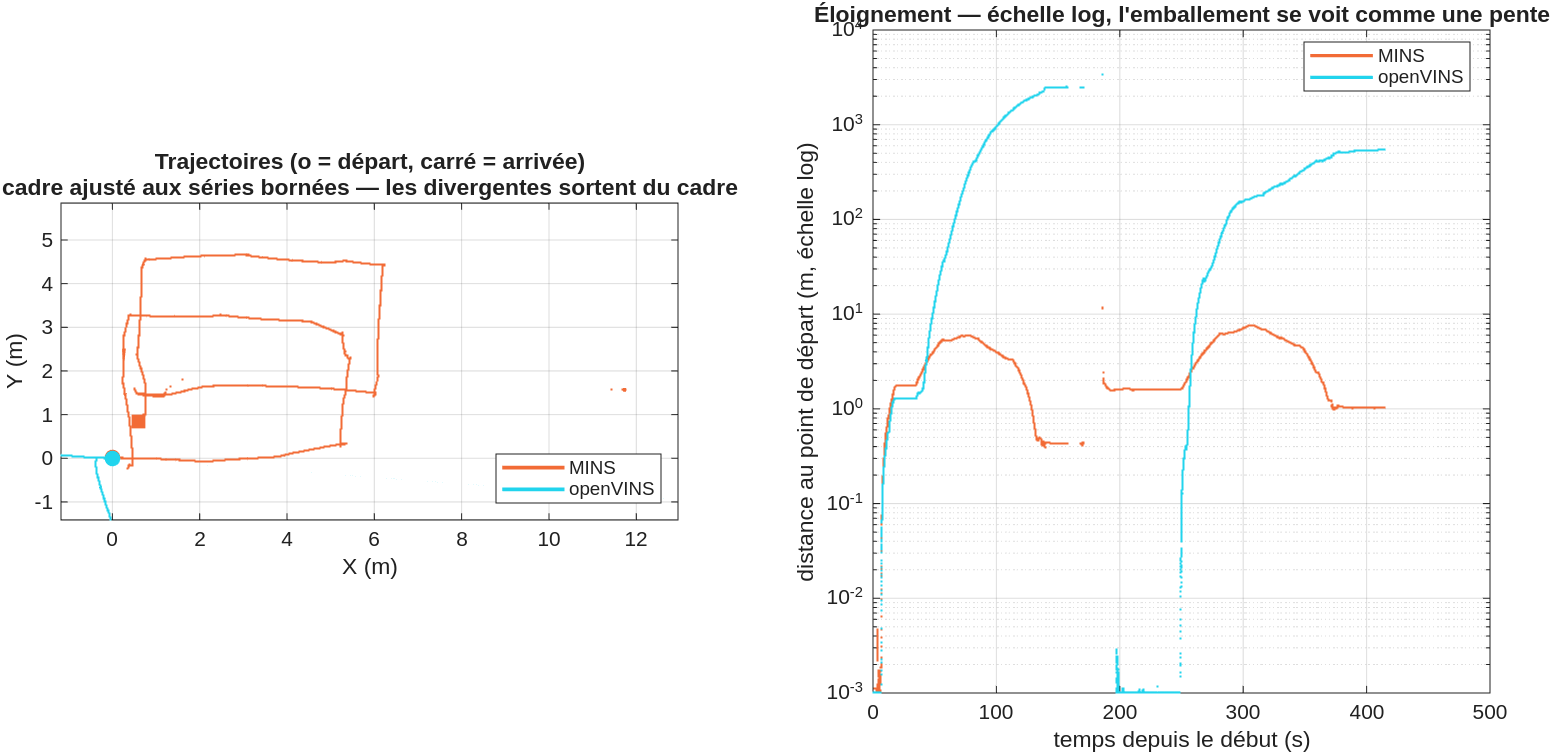
\includegraphics[width=\linewidth]{figures/estimators_comparison.png}%
  }{%
    \fbox{\parbox{0.9\linewidth}{\centering\vspace{1em}
    \code{figures/estimators\_comparison.png} not generated --- run
    \code{compare\_estimators('data/trajectories/zuptclean\_20260820\_162020')}
    \vspace{1em}}}%
  }
  \caption[MINS and openVINS on one recording]{MINS against openVINS on the
  same 600-second recording, so both estimators saw identical images and
  identical IMU samples. \textbf{Left:} $XY$ trajectories, circle marking the
  start and square the end. The frame is fitted to the \emph{bounded} series,
  so a diverging estimator leaves the frame rather than compressing everything
  else into a dot --- which is why only the MINS trace is visible here.
  \textbf{Right:} distance from the starting point against time, on a
  logarithmic $y$ axis, where an unbounded estimator reads as a rising slope.
  MINS stays within 1.78~m of its origin for the whole run and ends 1.40~m
  away; openVINS reaches 624.19~m and ends 559.22~m away. The gap is a factor
  of ${\approx}400$, which is why the two cannot share a linear axis.}
  \label{fig:estimators-comparison}
\end{figure}

Two cautions on how far this figure may be pushed. First, it establishes that
openVINS diverged \emph{on this recording}, not that it is inferior in
general: \S\ref{sec:openitems} records the starvation and ZUPT-threshold
faults that account for such runs, and several were still open on 2026-08-20.
Second, MINS staying bounded is not the same as MINS being correct. A frozen
initialisation holds a perfectly steady --- and perfectly wrong --- position,
and exactly that failure was observed on 2026-09-08 with $z$ locked
327~m below ground while $x$ and $y$ looked healthy. Boundedness is a
necessary condition here, never a sufficient one.

\section{Divergence across the whole recording set}
\label{sec:divsurvey}

Section~\ref{sec:estimator-comparison} compared the two estimators on one
recording. That is the only admissible way to claim one is better than the
other on a given run, but it says nothing about how \emph{often} either
fails. This section asks the second question against every paired recording
the campaign kept, and the answer is less flattering to both than the single
comparison suggests.

\subsection{An independent reference, and why the obvious metric is wrong}

Final distance from the origin is the tempting score and it is misleading
here. Three openVINS runs finish at $0.00$\,m, which reads as perfect
tracking; inspection shows two of them never left a $6$\,cm ball for the
whole recording, and a third excursioned $249$\,m before returning to the
start by coincidence. A stuck estimator and an accurate one are
indistinguishable by that number.

The bags carry \code{/firmware/wheel\_odom}, integrated from the encoders and
independent of both filters. Wheel odometry drifts --- that is why it is not
ground truth for accuracy --- but the question asked of it here is far
weaker and entirely within its competence: \emph{did the robot move, and
roughly how far}. Two recordings were discarded outright because the wheel
channel itself was corrupt, reporting path lengths of order
$10^{25}$\,m; \code{test2\_20260728\_142421} and
\code{test2\_20260805\_165507} are excluded on that basis, not on their
estimator behaviour. Fourteen paired recordings remain, ten with the robot
driving and four with it stationary.

\begin{figure}[htbp]
  \centering
  \IfFileExists{figures/divergence_par_essai.png}{%
    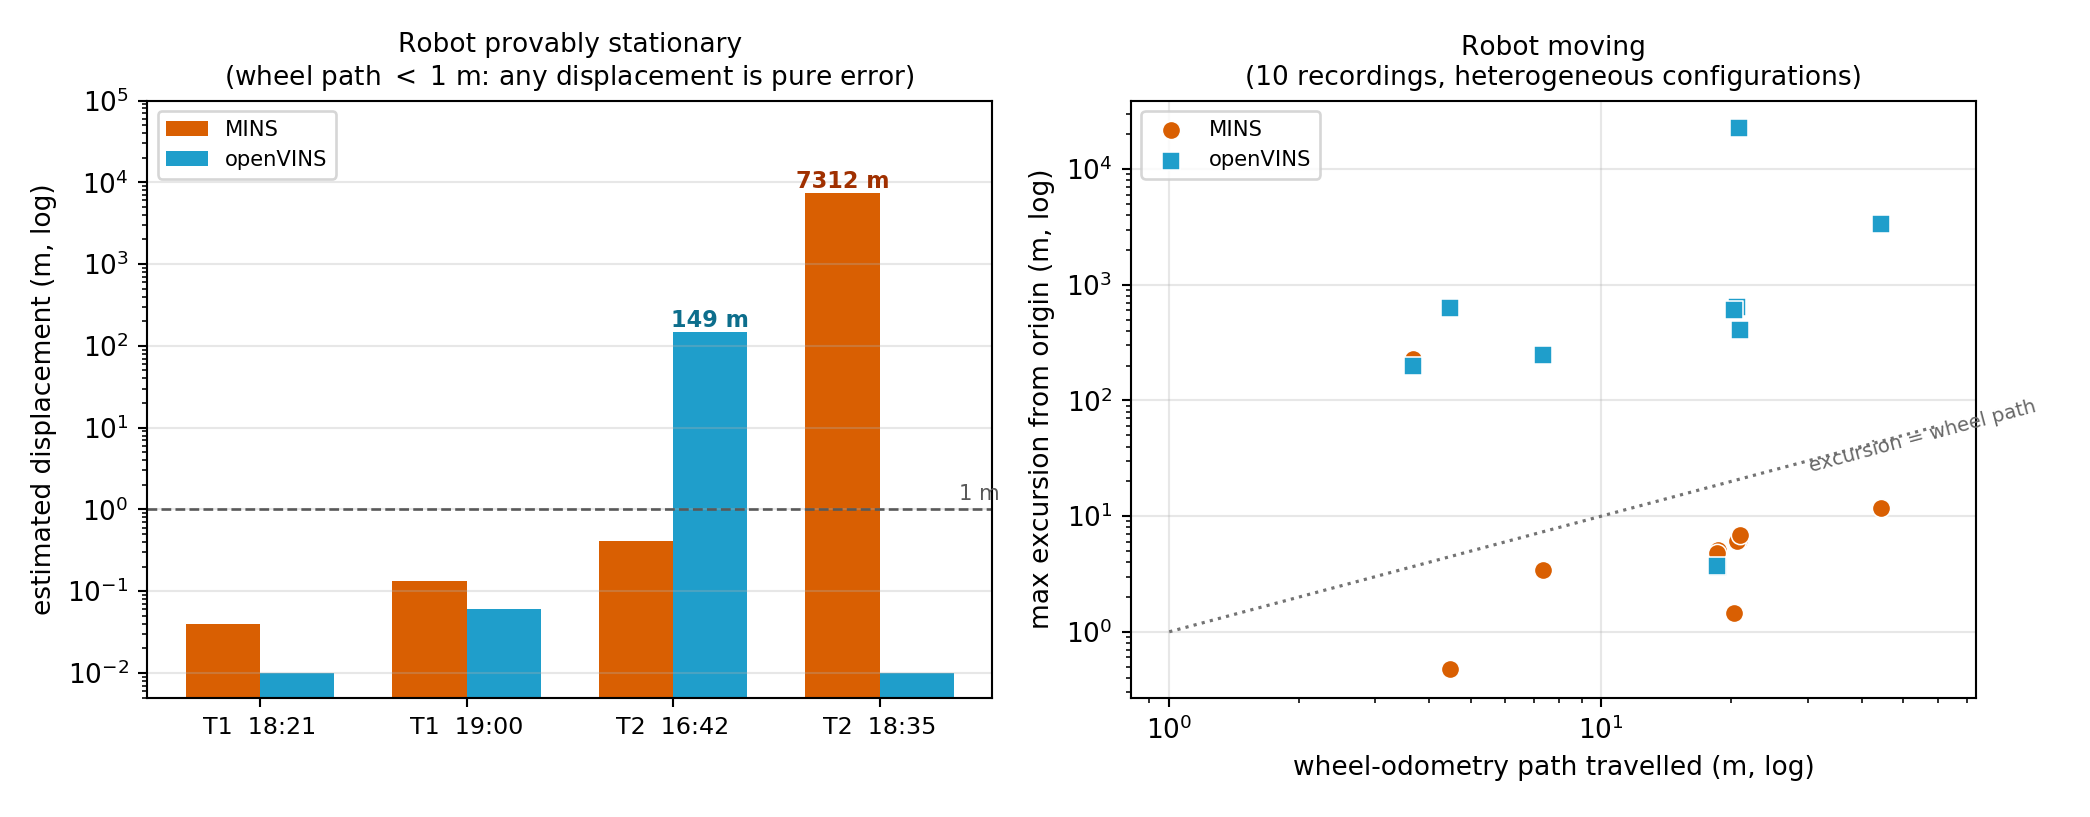
\includegraphics[width=\linewidth]{figures/divergence_par_essai.png}%
  }{%
    \fbox{\parbox{0.9\linewidth}{\centering\vspace{1em}
    \code{figures/divergence\_par\_essai.png} not generated
    \vspace{1em}}}%
  }
  \caption[Divergence across every paired recording]{Every paired recording
  in the campaign, classified by whether the wheels say the robot moved.
  \textbf{Left:} the four stationary runs. With a wheel path below 1\,m,
  \emph{any} estimated displacement is pure error, which makes these the
  cleanest test available. Each estimator produces exactly one catastrophic
  failure --- and not on the same run. \textbf{Right:} the ten driving runs,
  maximum excursion against distance actually travelled. The dotted line
  marks excursion equal to wheel path; a bounded estimator sits near or
  below it, since a closed indoor loop returns towards its start. MINS
  clusters there. openVINS sits two to four orders of magnitude above it on
  six of ten runs.}
  \label{fig:divergence-survey}
\end{figure}

\subsection{What the stationary runs show}

The left panel of Figure~\ref{fig:divergence-survey} is the result worth
keeping, because it needs no reference trajectory at all: the robot did not
move, so the correct answer is zero and every metre displayed is error.

\begin{center}
\begin{tabular}{@{}lrrr@{}}
\toprule
Recording & wheel path & MINS & openVINS \\
\midrule
\code{test1\_20260805\_182105} & $0.00$\,m & $0.04$\,m & $0.01$\,m \\
\code{test1\_20260805\_190028} & $0.05$\,m & $0.13$\,m & $0.06$\,m \\
\code{test2\_20260805\_164257} & $0.42$\,m & $0.41$\,m & $\mathbf{149.00}$\,m \\
\code{test2\_20260805\_183528} & $0.00$\,m & $\mathbf{7312.21}$\,m & $0.00$\,m \\
\bottomrule
\end{tabular}
\end{center}

\noindent Two runs are clean for both filters, at centimetre level. The
other two each contain one catastrophic failure, and they are different
runs: openVINS reports 149\,m of travel on a robot that moved 42\,cm, and
MINS reports \textbf{7.3\,km on a robot that did not move at all}.

That last figure is the sharpest evidence in this report for the
spontaneous-divergence item of \S\ref{sec:openitems}. It cannot be
attributed to bad odometry, to feature starvation during motion, or to an
aggressive manoeuvre, because there was no motion: the wheels recorded zero
path and zero peak velocity for the entire recording. Whatever fails,
fails with the platform standing still --- which is exactly what makes it
hard to reproduce deliberately and exactly why it is still open.

\subsection{What the driving runs show, and what they do not}

The right panel plots maximum excursion against wheel path. The dotted
diagonal is a useful reference rather than a bound: these are closed indoor
loops, so a sound estimator should end near where it started and its
excursion should not greatly exceed the distance travelled. MINS sits on or
below that line in nine of ten runs, with a single outlier at $230$\,m.
openVINS exceeds it by two to four orders of magnitude in six of ten,
reaching $2.3\times10^{4}$\,m.

\begin{trapbox}{What this survey is not}
It is not a controlled comparison. The fourteen recordings span 28 July to
20 August, and the configuration changed materially across that window ---
the ZUPT correction, the accelerometer scale, the wheel remapping and the
$\chi^2$ settings all moved. Several openVINS failures here are the ZUPT
verrou of \S\ref{sec:accelexpire}, since fixed. Nor is the sample
unbiased: these are the recordings that were kept, and a run abandoned
mid-way because something looked wrong is absent by construction.

The survey therefore supports a claim about \emph{failure modes} --- both
estimators possess an unbounded one, and it can fire with the robot
stationary --- and does not support a ranking. The controlled comparison of
\S\ref{sec:estimator-comparison}, one recording replayed through both, is
the only ranking evidence in this report.
\end{trapbox}

\section{The plausibility guard, measured against an independent reference}
\label{sec:gardemesuree}

\code{pose\_selector} carries a guard that freezes its output when the active
source jumps implausibly, and re-anchors when the source calms down. It was
written in July on the reasoning that no physically impossible jump should
reach the map, the trace or the return-to-base. Whether it \emph{works} had
never been quantified: the guard fires silently by design, and the fused
topic looks the same whether it is passing a healthy source through or
suppressing a catastrophic one.

Recording \code{zuptclean\_20260820\_162020} settles it, because it contains
the exact adversarial case. At $t = 97.94$\,s the operator switched the
served source to openVINS --- and on this run openVINS was diverging.

\begin{figure}[htbp]
  \centering
  \IfFileExists{figures/garde_vraisemblance.png}{%
    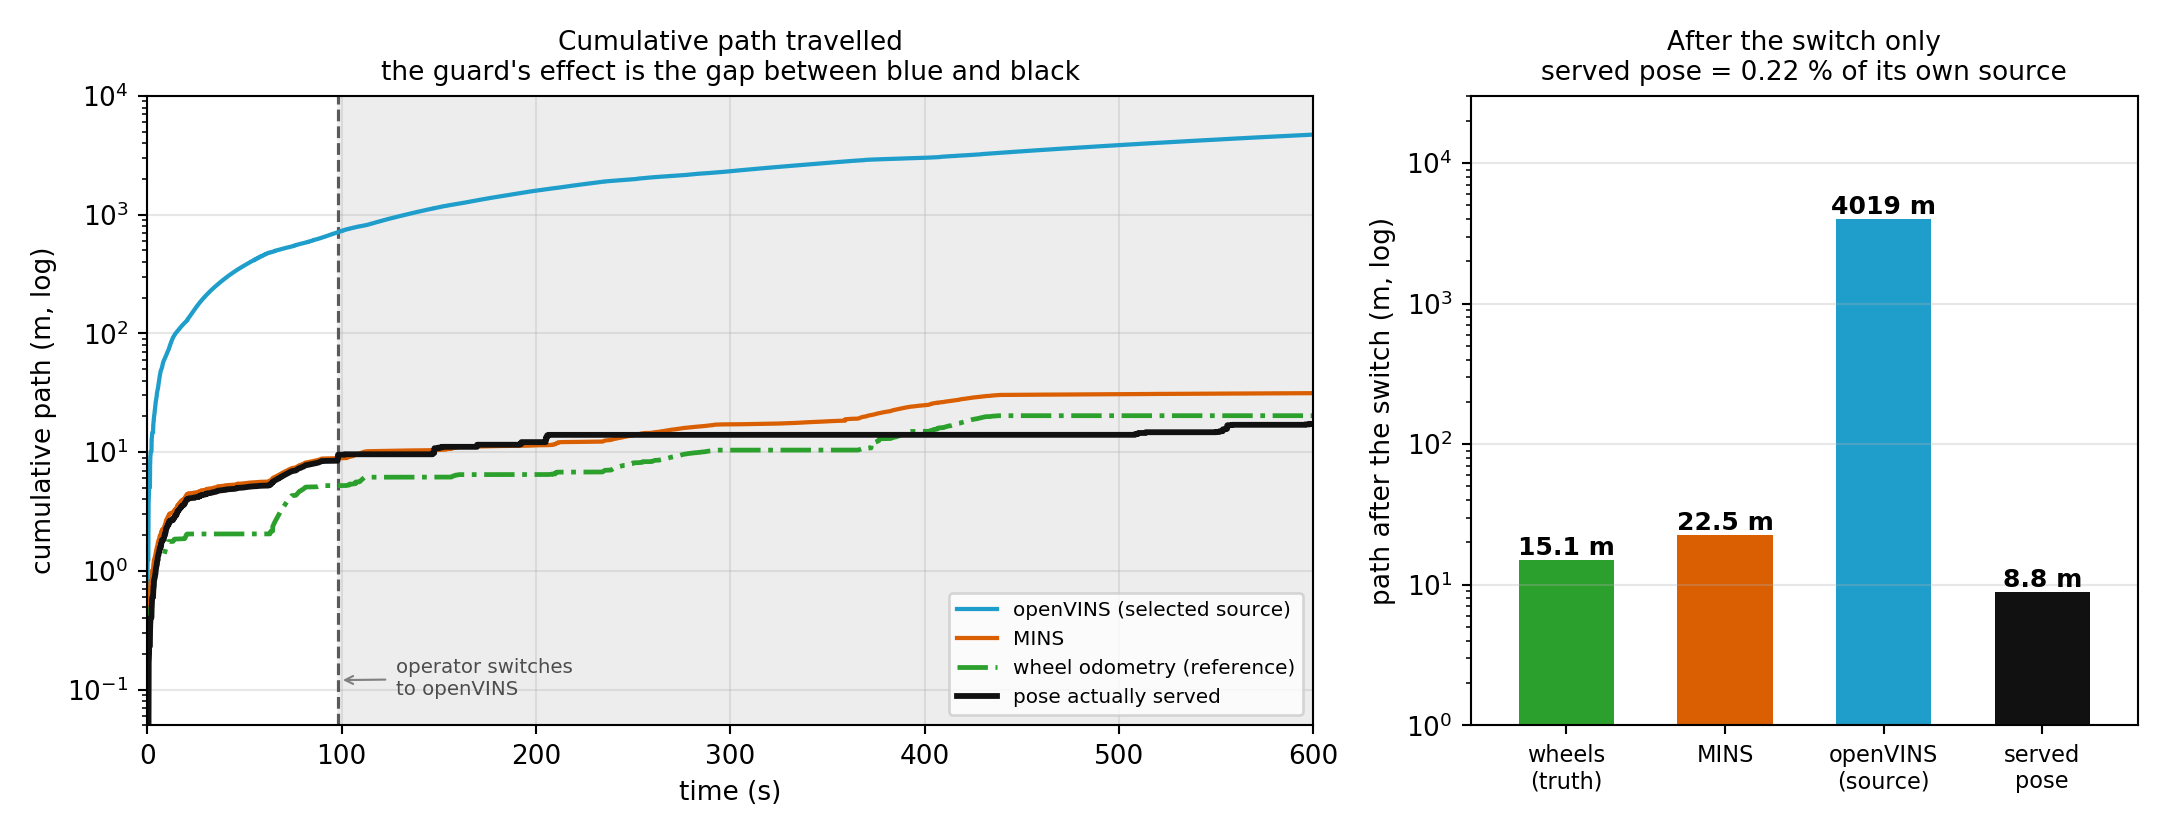
\includegraphics[width=\linewidth]{figures/garde_vraisemblance.png}%
  }{%
    \fbox{\parbox{0.9\linewidth}{\centering\vspace{1em}
    \code{figures/garde\_vraisemblance.png} not generated\vspace{1em}}}%
  }
  \caption[The plausibility guard suppressing a diverging source]{The guard
  under adversarial conditions, on a 600-second recording. \textbf{Left:}
  cumulative path travelled by each series, logarithmic. The dashed line
  marks the instant the operator selects openVINS as the served source; the
  shaded region is the interval during which a diverging estimator is the
  \emph{selected} one. The blue curve is what was asked for, the black curve
  is what was served, and the vertical gap between them is the guard's
  entire contribution. \textbf{Right:} path accumulated after the switch
  only. The served pose travels $8.8$\,m while the source it nominally
  follows travels $4019$\,m --- a suppression to $0.22\,\%$. Wheel odometry,
  independent of both estimators, gives $15.1$\,m as the reference.}
  \label{fig:garde-mesuree}
\end{figure}

\subsection{What the numbers establish}

Over the interval where openVINS was the selected source:

\begin{center}
\begin{tabular}{@{}lrl@{}}
\toprule
Series & path after switch & role \\
\midrule
wheel odometry      & $15.1$\,m   & independent reference \\
MINS                & $22.5$\,m   & running, not selected$^{\dagger}$ \\
openVINS            & $4019.5$\,m & \textbf{selected source} \\
pose served         & $8.8$\,m    & what reached the map \\
\bottomrule
\end{tabular}
\end{center}

\noindent $^{\dagger}$ MINS's $22.5$\,m against the wheels' $15.1$\,m is
\emph{not} a $49\,\%$ estimation error; it is largely the sampling-rate
artefact quantified in \S\ref{sec:cadencetrap}. At matched rates the two
agree to about two per cent.

\noindent The operator selected a broken estimator and the map stayed
sane. Four kilometres of accumulated nonsense produced under nine metres of
served motion, against a true fifteen. Expressed as a ratio the guard
suppressed $99.78\,\%$ of its own source's path, and it did so without any
supervisory signal telling it that openVINS had failed --- the decision is
taken from the pose stream alone, one sample at a time.

\subsection{The cost, which the same numbers make visible}

The served path of $8.8$\,m sits \emph{below} the wheel reference of
$15.1$\,m, and that shortfall is not noise. It is the guard's price, and it
follows directly from what freezing means: while the output is held, the
robot's real motion is not tracked. Roughly six metres of genuine
displacement were lost in that recording --- served as stillness rather than
as motion.

This is the correct trade for the purpose the guard was written for. A
frozen pose is wrong by a bounded amount that shrinks the moment the source
recovers; a passed-through divergence is wrong without bound and pollutes
the trace, the logged trajectory and any return-to-base computed from it.
But the trade must be stated, because a reader comparing the served path
against ground truth would otherwise read the $6$\,m deficit as an
estimation error rather than as the guard doing precisely its job.

\begin{trapbox}{Two things this recording does not show}
\textbf{It does not rank the estimators.} openVINS diverged here for
reasons documented in \S\ref{sec:accelexpire} and since corrected; a
recording from before a fix is evidence about the guard, not about the
estimator's present quality.

\textbf{It does not validate the guard's thresholds.} What is measured is
that the guard fires and suppresses on \emph{this} magnitude of divergence
--- four kilometres against a $0.21$\,m/s platform, which is not a subtle
case. A divergence slow enough to stay under
\code{max\_plausible\_speed} would pass through untouched, and nothing in
this recording says how slow that is. The guard is demonstrated against a
gross failure; its behaviour near its own threshold remains uncharacterised.
\end{trapbox}

\subsection{The stationarity detector, validated in the direction that matters}
\label{sec:zuptvalid}

The same recording carries \code{/imu\_sanitizer/is\_stationary}, the boolean
that gates zero-velocity updates. It is a safety-critical signal in one
direction only, and the asymmetry is worth naming before any number is
quoted. Declaring the platform stationary when it is moving injects a false
zero-velocity constraint into a filter that has no way to contradict it ---
the error is asserted, not merely missed. Declaring motion when the platform
is still merely forgoes a ZUPT opportunity: the filter loses information it
could have had, but is told nothing false.

A single detector accuracy figure therefore hides the only question that
matters. Scored against wheel odometry over the same recording, weighting by
time rather than by transition count so that brief flickers do not dominate:

\begin{center}
\begin{tabular}{@{}lrrl@{}}
\toprule
Detector says & wheels say & time & consequence \\
\midrule
stationary & stationary & $345.5$\,s  ($60.2\,\%$) & correct \\
moving     & moving     & $127.3$\,s  ($22.2\,\%$) & correct \\
stationary & \textbf{moving} & $\mathbf{0.0}$\,\textbf{s}  ($0.0\,\%$) & \textbf{false ZUPT} \\
moving     & stationary & $101.0$\,s  ($17.6\,\%$) & ZUPT opportunity lost \\
\bottomrule
\end{tabular}
\end{center}

\noindent Overall temporal agreement is $82.4\,\%$, which taken alone would
read as mediocre. The decomposition says something quite different: the
$17.6\,\%$ disagreement lies \emph{entirely} in the benign direction, and
the dangerous cell is empty. Over $574$\,s of classified time the detector
never once asserted stationarity while the wheels were turning.

Of the $447$\,s during which the platform was genuinely still, the detector
recognised $77.4\,\%$ and missed $22.6\,\%$. That is the cost of its
conservatism, and it is the right side to err on: a missed ZUPT leaves the
filter no worse than a filter without ZUPT at all, whereas a false ZUPT is
an actively wrong measurement. The zero in the third row is the result;
the $82.4\,\%$ is not.

\begin{trapbox}{Scope of this validation}
One recording, one motion profile, one lighting condition. The detector's
thresholds were not exercised near their boundaries: this run alternates
between clear stops and clear driving at up to $0.21$\,m/s, so the
interesting regime --- creeping motion just above the detector's own
threshold --- is absent from the data entirely. What is established is that
the detector has no gross false-positive failure mode on ordinary
stop-and-go operation, not that it is correct near its decision boundary.
The $26$\,s excluded from the table are intervals where the wheel window
held too few samples to classify, and are reported here rather than
silently dropped.
\end{trapbox}

\subsection{The sampling-rate inflation, measured}
\label{sec:cadencetrap}

The table above lists MINS at $22.5$\,m where the wheels give $15.1$\,m, and
that juxtaposition invites a conclusion it does not support.
\S\ref{sec:july29extent} derives why: cumulative path length sums $n$
increments, each collecting its own independent noise, and the resulting
inflation is \emph{quadratic in the sampling rate}. Two series describing the
same trajectory at different rates are therefore not comparable as path
lengths at all --- and MINS publishes at ${\approx}86$\,Hz against
${\approx}20$\,Hz for \code{/firmware/wheel\_odom}, a ratio of $4.3$.

That derivation has not, until now, been checked against data. The test is
direct: decimate MINS to the wheel rate and recompute. Across six recordings
in which both series are healthy:

\begin{center}
\begin{tabular}{@{}lrrr@{}}
\toprule
Recording & wheels & MINS at 86\,Hz & MINS at 20\,Hz \\
\midrule
\code{test1\_20260728\_133541} & $20.81$ & $25.40$ & $23.84$ \\
\code{test1\_20260729\_145637} & $18.60$ & $16.78$ & $15.44$ \\
\code{test1\_20260805\_184025} & $20.57$ & $21.24$ & $19.57$ \\
\code{test1\_20260805\_191300} & $20.99$ & $23.35$ & $22.00$ \\
\code{test2\_20260729\_145417} & $18.57$ & $16.38$ & $15.11$ \\
\code{zuptclean\_20260820\_162020} & $20.28$ & $23.22$ & $20.28$ \\
\midrule
\textbf{median ratio to wheels} & --- & $\mathbf{1.07}$ & $\mathbf{0.98}$ \\
\bottomrule
\end{tabular}
\end{center}

\noindent Decimation moves the median ratio from $1.07$ to $0.98$. At
matched rates MINS and wheel odometry agree on distance travelled to within
about two per cent, across six independent recordings --- and since the two
references are physically unrelated, one inertial-visual and one from wheel
encoders, that agreement says something neither could say alone. The
apparent excess at full rate is the predicted artefact, now observed.

\begin{trapbox}{What this does and does not license}
It licenses the statement that MINS's \emph{scale} is sound: over twenty
metres of driving it neither stretches nor shrinks the path appreciably
against an independent odometric reference.

It does not license a claim about \emph{accuracy}. Two trajectories can have
identical lengths and diverge steadily in position; path length is blind to
heading error, which is precisely the channel this platform is weakest in
(\S\ref{sec:wheelyaw}) and which \S\ref{sec:capdesaccord} takes up next. Nor
is the wheel reference itself exact: the effective radius carries a
calibrated $r_{\mathrm{eff}} = 62.2$\,mm against a stock $62.5$\,mm, and
mecanum rollers scrub. The two per cent should be read as ``no gross scale
error detected'', not as a measured accuracy.
\end{trapbox}

\subsection{Heading: two references that disagree, and neither is truth}
\label{sec:capdesaccord}

The previous subsection established that MINS's path \emph{length} agrees
with wheel odometry to two per cent, and closed by noting that length is
blind to heading. This one looks at heading directly, and the result is
less comfortable.

Unwrapping both yaw signals from a common origin and comparing accumulated
rotation at the end of each recording:

\begin{center}
\begin{tabular}{@{}lrrrr@{}}
\toprule
Recording & $|{\rm rot}|$ wheels & duration & disagreement & per rotation \\
\midrule
\code{test1\_20260728\_133541}  & $758^\circ$  & $928$\,s & $22.0^\circ$ & $2.90\,\%$ \\
\code{test1\_20260729\_145637}  & $535^\circ$  & $129$\,s & $15.9^\circ$ & $2.98\,\%$ \\
\code{test1\_20260805\_184025}  & $511^\circ$  & $163$\,s & $42.6^\circ$ & $8.34\,\%$ \\
\code{test1\_20260805\_191300}  & $600^\circ$  & $213$\,s & $44.0^\circ$ & $7.32\,\%$ \\
\code{test2\_20260729\_145417}  & $509^\circ$  & $137$\,s & $22.8^\circ$ & $4.48\,\%$ \\
\code{zuptclean\_20260820\_162020} & $2052^\circ$ & $600$\,s & $92.7^\circ$ & $4.52\,\%$ \\
\bottomrule
\end{tabular}
\end{center}

\noindent Two things are solid. The disagreement is \textbf{systematically
one-signed} --- MINS reports more accumulated rotation than the wheels in
all six recordings, never less --- and it is \textbf{large}: a median
$4.5\,\%$ of cumulative rotation, or equivalently ${\approx}10^\circ$ per
minute of operation. On runs that amount to roughly one full turn, the two
references end tens of degrees apart.

\paragraph{The discrimination fails, and that is the finding.}
The obvious next question is whether this is a \emph{scale} error, which
would scale with rotation, or a \emph{drift}, which would scale with time.
Normalising by each and comparing dispersion:
\begin{equation}
\mathrm{CV}\bigl(\text{per rotation}\bigr) = 0.41,
\qquad
\mathrm{CV}\bigl(\text{per unit time}\bigr) = 0.47 .
\end{equation}
The rotation hypothesis is marginally more stable, and the margin is far too
thin to conclude from. Both normalisations leave a spread of nearly a factor
of three ($2.90\,\%$ to $8.34\,\%$; $1.4$ to $15.7^\circ$/min). No single
mechanism explains these six recordings. The likely reading is that both
contribute and that configuration heterogeneity across the campaign
dominates either --- but that is a hypothesis, and it is recorded here as
one.

\begin{trapbox}{Why this cannot be resolved with the sensors on the rover}
It is tempting to declare the wheels right and MINS wrong, or the reverse.
Neither is available. The wheel heading applies a $1.76$ scrub
compensation calibrated for rubber tyres to mecanum rollers that do not
scrub (\S\ref{sec:wheelyaw}) --- the report's own analysis says that number
is wrong for this hardware. MINS's heading is the channel this campaign has
repeatedly identified as its weakest. The comparison therefore places a
bound on their \emph{mutual} consistency and cannot attribute the error.

What it does establish is a requirement: closing this question needs a
heading reference independent of both, and the platform does not carry one.
The magnetometer on the incoming MinIMU-9 v5 is the first candidate the
project will have had --- which is a further reason to characterise that
sensor properly rather than treat it as a spare accelerometer.
\end{trapbox}

\section{A validity test that needs no reference at all}
\label{sec:plafondphysique}

Every comparison so far has needed something to compare against --- another
estimator, wheel odometry, a closed loop. There is one test that needs
nothing: the platform cannot exceed its own maximum speed. The LEO Rover is
geared to roughly $0.4$\,m/s and has been measured at $0.21$\,m/s in normal
operation. Any estimator reporting more than that is wrong, and no ground
truth is required to say so.

The four recordings of 2026-08-21 in \code{data/matlab/} carry all three
estimators simultaneously, with velocity and full pose covariance --- the
only set in this campaign that does. Three are short stationary tests, the
fourth is a seven-minute drive.

\begin{figure}[htbp]
  \centering
  \IfFileExists{figures/plafond_physique.png}{%
    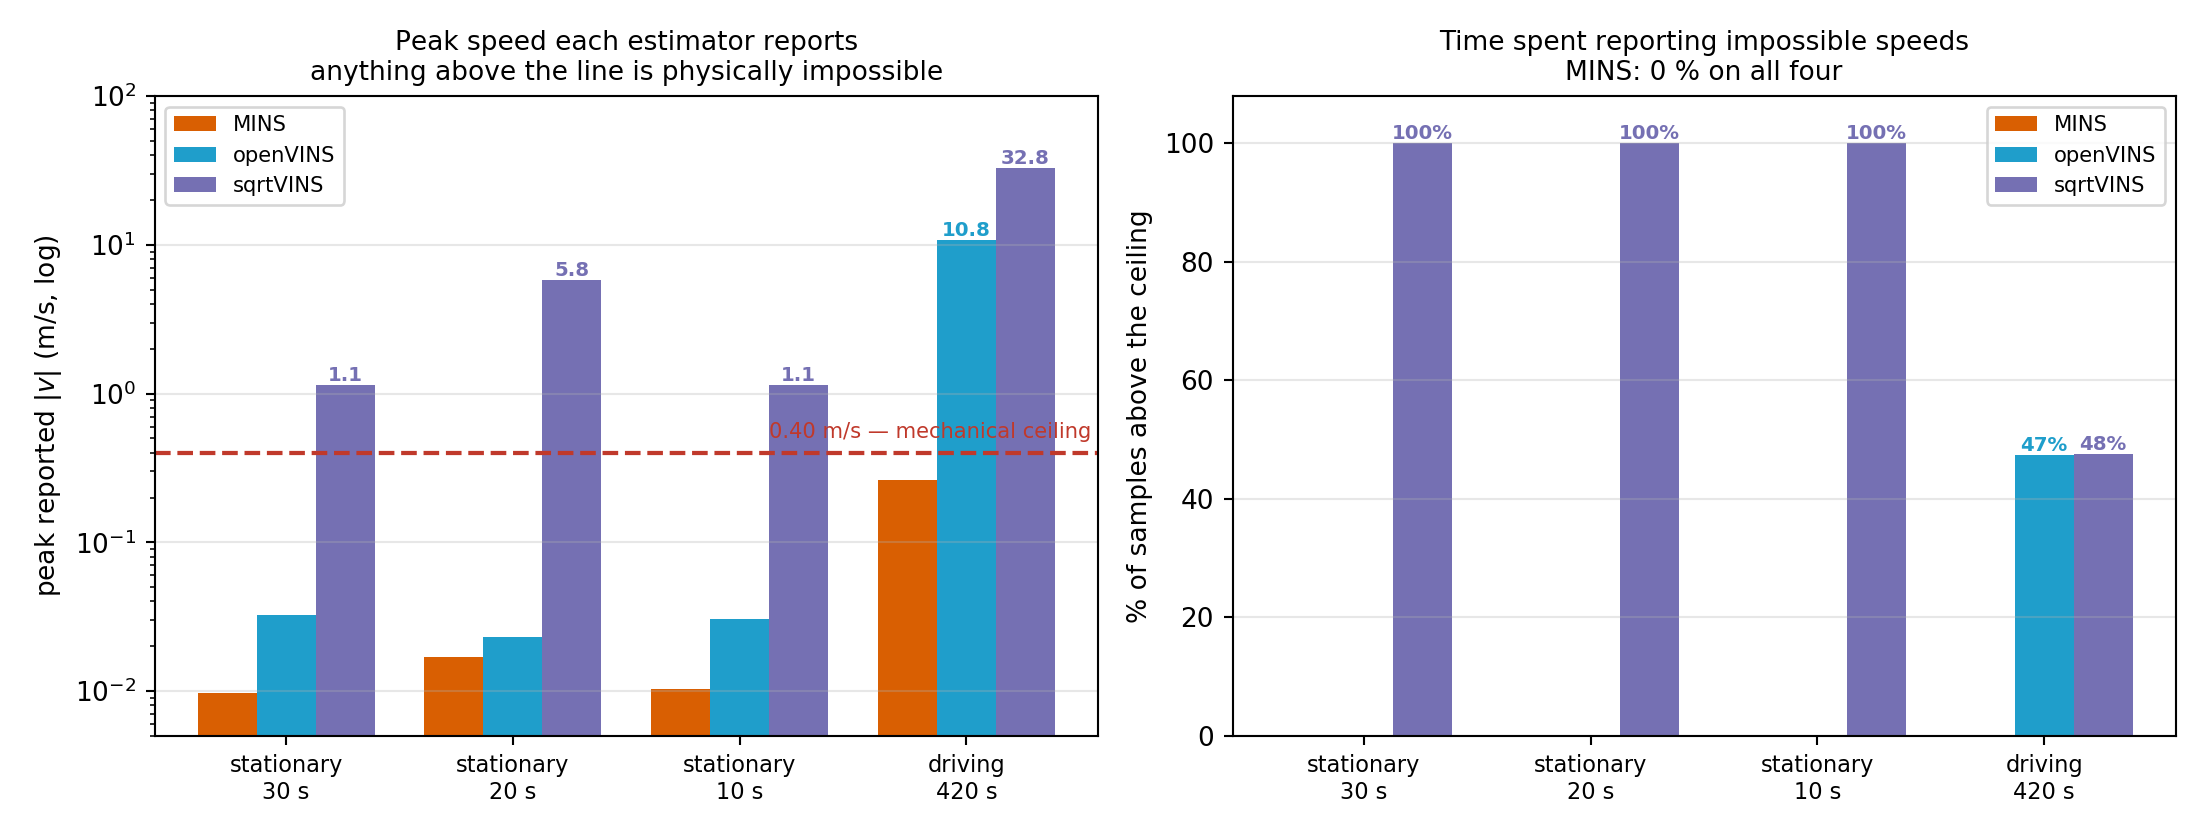
\includegraphics[width=\linewidth]{figures/plafond_physique.png}%
  }{%
    \fbox{\parbox{0.9\linewidth}{\centering\vspace{1em}
    \code{figures/plafond\_physique.png} not generated\vspace{1em}}}%
  }
  \caption[Reported speed against the platform's mechanical ceiling]{The
  three estimators against a constraint none of them can argue with.
  \textbf{Left:} peak reported speed, logarithmic; the dashed line is the
  rover's $0.4$\,m/s mechanical ceiling and everything above it is
  impossible by construction. \textbf{Right:} the fraction of samples above
  that ceiling. MINS does not appear in the right panel because its bar is
  zero on all four recordings.}
  \label{fig:plafond}
\end{figure}

\subsection{What the three estimators do with an impossible claim}

\begin{center}
\begin{tabular}{@{}llrr@{}}
\toprule
Recording & estimator & peak $|v|$ & \% above ceiling \\
\midrule
stationary, 30\,s & MINS & $0.010$ & $0.0\,\%$ \\
                  & openVINS & $0.032$ & $0.0\,\%$ \\
                  & sqrtVINS & $1.148$ & $\mathbf{100.0\,\%}$ \\
\midrule
stationary, 20\,s & MINS & $0.017$ & $0.0\,\%$ \\
                  & openVINS & $0.023$ & $0.0\,\%$ \\
                  & sqrtVINS & $\mathbf{5.779}$ & $\mathbf{100.0\,\%}$ \\
\midrule
stationary, 10\,s & MINS & $0.010$ & $0.0\,\%$ \\
                  & openVINS & $0.030$ & $0.0\,\%$ \\
                  & sqrtVINS & $1.147$ & $\mathbf{100.0\,\%}$ \\
\midrule
driving, 420\,s   & MINS & $0.264$ & $0.0\,\%$ \\
                  & openVINS & $10.839$ & $47.5\,\%$ \\
                  & sqrtVINS & $\mathbf{32.835}$ & $47.6\,\%$ \\
\bottomrule
\end{tabular}
\end{center}

\noindent MINS is inside the envelope on every sample of every recording,
including a peak of $0.264$\,m/s on the drive that sits sensibly below the
ceiling. That is a stronger statement than any comparison against another
estimator, because it cannot be argued with: the platform could not have
done what the other two describe.

\subsection{Dating the sqrtVINS result, which changes what it means}

Reading the table as a ranking would be wrong, and the dates say why.
These recordings are from the evening of 2026-08-21. The
\code{02\_zupt\_guards} patch --- the one that removed the
\code{!disparity\_passed \&\&} short-circuit, measured at 290 acceptances
against 0 rejections with $|v| = 1.0\times10^{23}$\,m/s --- is dated
2026-08-24, three days later.

What Figure~\ref{fig:plafond} shows for sqrtVINS is therefore not its
current behaviour. It is a measurement of \emph{the defect that patch
corrected}, taken before the correction existed, and it is worth keeping for
exactly that reason: the bug report describes a $\chi^2$ gate that never
rejected, and this is what that looks like from the outside --- a filter
reporting $5.8$\,m/s on a platform standing still, for one hundred per cent
of a twenty-second recording.

openVINS is a different matter. It is not covered by that patch, it is
clean on all three stationary recordings, and it spends $47.5\,\%$ of the
seven-minute drive above the ceiling. That behaviour is not dated away by
anything in this campaign.

\subsection{The covariance is not always honest either}

These files also carry each filter's own $3\sigma$ bounds, which allows a
question asked nowhere else in this report: does the uncertainty an
estimator reports actually contain its error?

On the 20-second stationary recording, sqrtVINS ends $0.151$\,m from where
it started while reporting a final $3\sigma$ of $0.063$\,m. The error
exceeds by a factor of $2.4$ the interval the filter claims contains the
truth with $99.7\,\%$ probability. That is overconfidence, and it is more
dangerous than a large error honestly declared: a consumer weighting this
pose by its stated covariance would trust it far more than it deserves.

The other two err the opposite way on the same recordings. MINS reports
$3\sigma$ between $1.1$ and $1.4$\,m for closure errors of $3$ to $8$\,mm
--- conservative by two orders of magnitude --- and openVINS reports
$0.26$\,m for millimetre closures. Neither is well calibrated; but a filter
that overstates its uncertainty degrades gracefully, while one that
understates it invites exactly the trust it cannot support.

\begin{trapbox}{Why the ceiling test deserves to be automated}
\code{pose\_selector} already computes this quantity: its
\code{max\_plausible\_speed} guard exists to freeze the output when a source
claims impossible motion, and \S\ref{sec:gardemesuree} measured it
suppressing a 4\,km divergence. What the present section adds is that the
same threshold is a \emph{diagnostic}, not only a filter. The fraction of
samples above the ceiling is computable offline from any recording, needs
no reference trajectory, and separates the three estimators cleanly here.
It costs nothing to log and would have flagged the sqrtVINS defect on the
first recording rather than three days later.
\end{trapbox}

\section{Is the filter honest about its own uncertainty?}
\label{sec:nees}

An estimator publishes two things: a state and a covariance. Every
consumer downstream --- a fusion node, a $\chi^2$ gate, a planner deciding
whether it knows where it is --- weights the first by the second. This
report has measured the first extensively and has never once checked the
second. This section does, and the answer differs by three orders of
magnitude between estimators.

\subsection{The test, and why a stationary robot makes it exact}

Consistency has a standard definition. For an estimate $\hat{\mathbf{x}}$
of a true state $\mathbf{x}$ with reported covariance $\mathbf{P}$, the
\emph{normalized estimation error squared} is
\begin{equation}
\varepsilon \;=\; \tilde{\mathbf{x}}^{\top}\mathbf{P}^{-1}\tilde{\mathbf{x}},
\qquad \tilde{\mathbf{x}} = \hat{\mathbf{x}} - \mathbf{x} .
\label{eq:nees}
\end{equation}
If the filter's error is genuinely zero-mean Gaussian with covariance
$\mathbf{P}$ --- which is exactly what publishing $\mathbf{P}$ asserts ---
then $\varepsilon$ follows a chi-squared law with as many degrees of freedom
as the state has dimensions. Restricting to the $3\times3$ position block:
\begin{equation}
\varepsilon \;\sim\; \chi^2(3),
\qquad
\mathbb{E}[\varepsilon] = 3,
\qquad
\mathrm{med}(\varepsilon) = 2.366,
\qquad
F^{-1}(0.95) = 7.815 .
\label{eq:chi3}
\end{equation}
A median far below $2.37$ means $\mathbf{P}$ is too large --- the filter
declares more uncertainty than it has. A median far above means
$\mathbf{P}$ is too small, and the filter is claiming a precision it does
not possess.

Applying Eq.~(\ref{eq:nees}) normally requires ground truth, which this
platform does not have. The stationary recordings remove that obstacle
entirely: if the robot does not move, its true position is its initial
position, exactly and by construction, so
\begin{equation}
\tilde{\mathbf{p}}(t) \;=\; \hat{\mathbf{p}}(t) - \hat{\mathbf{p}}(0)
\end{equation}
is the error itself, not an approximation of it. The three short recordings
of 2026-08-21 are therefore the only place in this campaign where
Eq.~(\ref{eq:nees}) can be evaluated without assumption.

\begin{center}
\begin{tikzpicture}[font=\small,
  vraie/.style={draw=green!45!black, thick},
  annonce/.style={draw=alertred!70, thick, dashed}]
  % cas 1 : conservateur
  \begin{scope}[shift={(0,0)}]
    \node[font=\scriptsize\bfseries] at (0,1.75) {conservative};
    \draw[annonce] (0,0) ellipse (1.35 and 1.05);
    \draw[vraie]   (0,0) ellipse (0.16 and 0.13);
    \foreach \x/\y in {0.05/0.03, -0.06/0.05, 0.03/-0.07, -0.04/-0.03, 0.07/0.01}
      \fill[black!70] (\x,\y) circle (0.9pt);
    \node[font=\scriptsize, text=alertred!80] at (0,-1.42) {$\varepsilon \ll 2.37$};
  \end{scope}
  % cas 2 : coherent
  \begin{scope}[shift={(3.9,0)}]
    \node[font=\scriptsize\bfseries] at (0,1.75) {calibrated};
    \draw[annonce] (0,0) ellipse (0.85 and 0.65);
    \foreach \x/\y in {0.35/0.22, -0.42/0.31, 0.28/-0.44, -0.55/-0.18, 0.62/0.09, -0.2/0.5}
      \fill[black!70] (\x,\y) circle (0.9pt);
    \node[font=\scriptsize, text=green!35!black] at (0,-1.42) {$\varepsilon \approx 2.37$};
  \end{scope}
  % cas 3 : surconfiant
  \begin{scope}[shift={(7.8,0)}]
    \node[font=\scriptsize\bfseries] at (0,1.75) {overconfident};
    \draw[annonce] (0,0) ellipse (0.30 and 0.24);
    \foreach \x/\y in {0.95/0.55, -1.05/0.68, 0.75/-0.9, -1.2/-0.35, 1.25/0.15}
      \fill[black!70] (\x,\y) circle (0.9pt);
    \node[font=\scriptsize, text=alertred!80] at (0,-1.42) {$\varepsilon \gg 7.81$};
  \end{scope}
  \node[font=\scriptsize, anchor=west] at (-1.9,-2.15)
    {dashed: the $\mathbf{P}$ the filter publishes \quad dots: where its error actually lands};
\end{tikzpicture}
\end{center}

\subsection{Result}

Evaluating Eq.~(\ref{eq:nees}) sample by sample, discarding the first tenth
of each recording as initialisation transient:

\begin{center}
\begin{tabular}{@{}llrrl@{}}
\toprule
Recording & estimator & median $\varepsilon$ & $\sigma$ factor & assessment \\
\midrule
stationary 30\,s & MINS     & $0.0003$ & $0.011$ & far too large \\
                 & openVINS & $0.0001$ & $0.007$ & far too large \\
                 & sqrtVINS & $0.0920$ & $0.197$ & too large \\
\midrule
stationary 20\,s & MINS     & $0.0006$ & $0.016$ & far too large \\
                 & openVINS & $0.0000$ & $0.005$ & far too large \\
                 & sqrtVINS & $\mathbf{45.75}$ & $\mathbf{4.39}$ & \textbf{overconfident} \\
\midrule
stationary 10\,s & MINS     & $0.0000$ & $0.004$ & far too large \\
                 & openVINS & $0.0001$ & $0.008$ & far too large \\
                 & sqrtVINS & $0.1471$ & $0.249$ & too large \\
\bottomrule
\end{tabular}
\end{center}

\noindent The fourth column restates the third in units an implementer can
act on. Since $\varepsilon$ is quadratic in the error and inversely
quadratic in $\sigma$, a median NEES of $\varepsilon_m$ corresponds to a
reported standard deviation wrong by the factor
\begin{equation}
k \;=\; \sqrt{\frac{\varepsilon_m}{\mathrm{med}\,\chi^2(3)}}
  \;=\; \sqrt{\frac{\varepsilon_m}{2.366}} ,
\label{eq:sigmafactor}
\end{equation}
with $k<1$ meaning $\sigma$ is inflated and $k>1$ meaning it is deflated.


\begin{figure}[htbp]
  \centering
  \IfFileExists{figures/nees_coherence.png}{%
    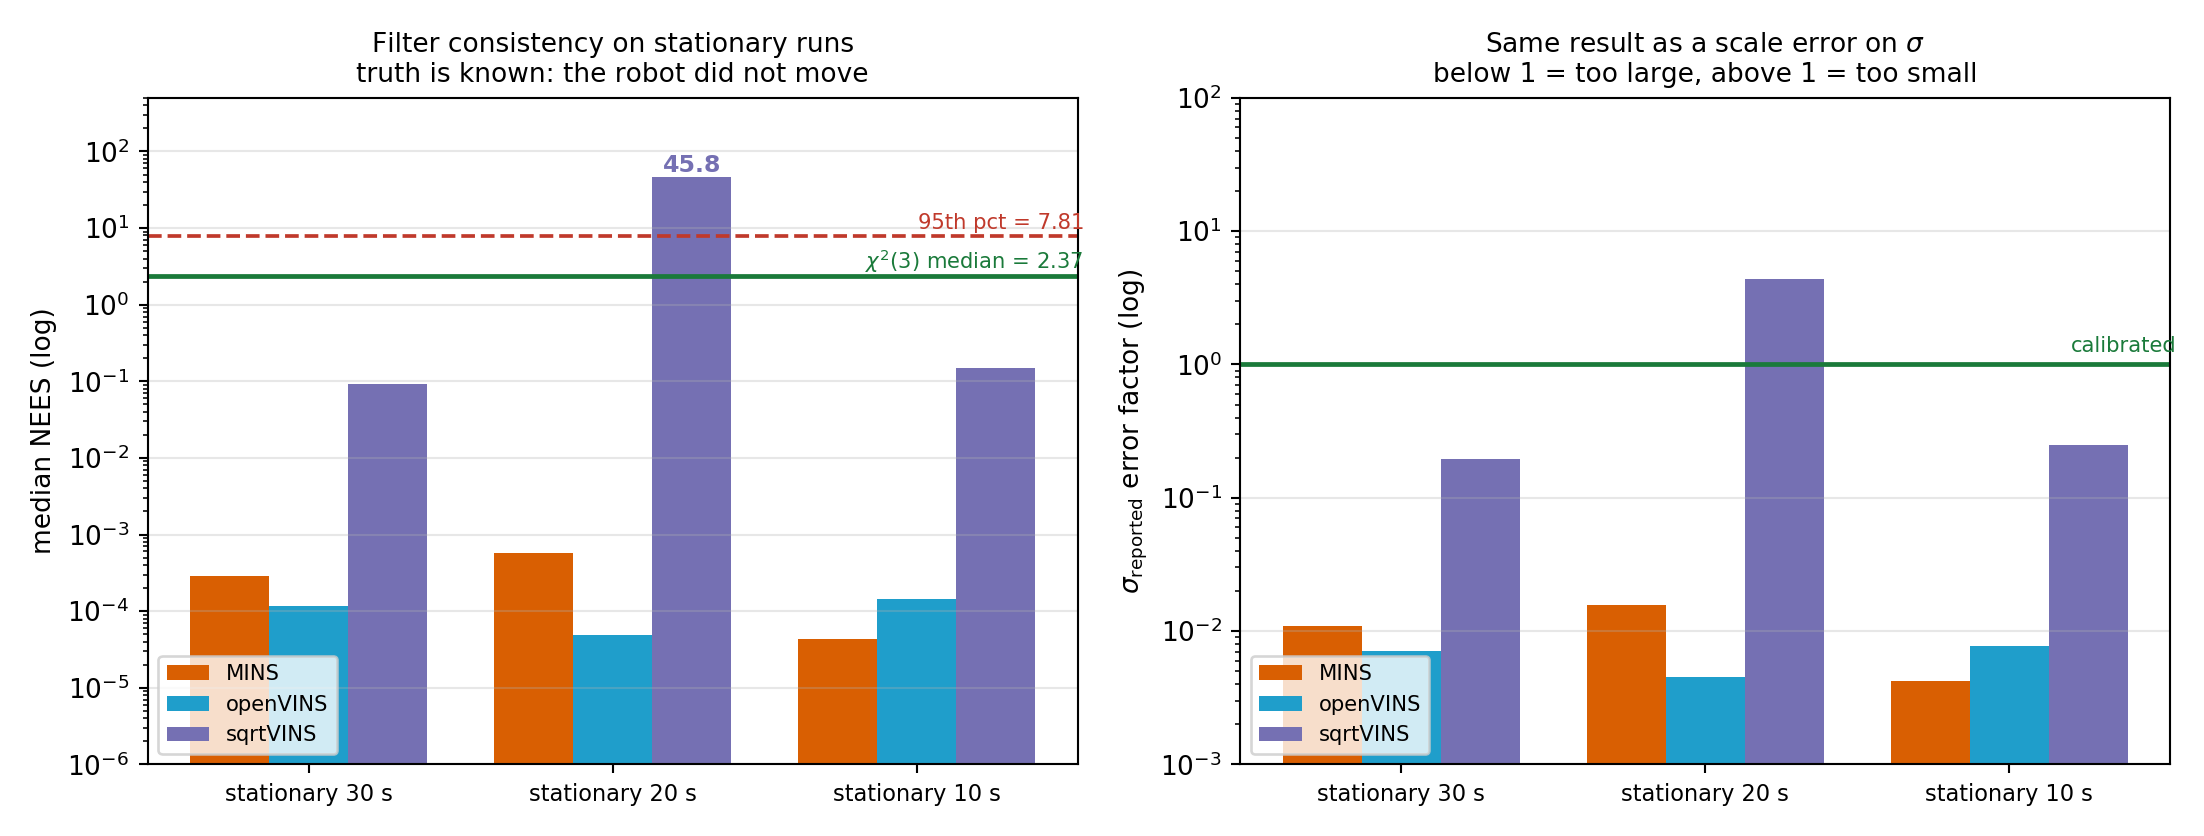
\includegraphics[width=\linewidth]{figures/nees_coherence.png}%
  }{%
    \fbox{\parbox{0.9\linewidth}{\centering\vspace{1em}
    \code{figures/nees\_coherence.png} not generated\vspace{1em}}}%
  }
  \caption[Filter consistency against the $\chi^2(3)$ reference]{Consistency
  on the three stationary recordings, where the true position is known
  exactly. \textbf{Left:} median NEES, logarithmic, against the $\chi^2(3)$
  median of $2.37$ (solid) and its $95$th percentile of $7.81$ (dashed).
  MINS and openVINS sit four orders of magnitude below the reference;
  sqrtVINS exceeds the $95$th percentile on one run. \textbf{Right:} the
  same result expressed by Eq.~(\ref{eq:sigmafactor}) as a multiplicative
  error on the reported $\sigma$, where unity is calibrated.}
  \label{fig:nees}
\end{figure}

\subsection{Reading the two failure modes}

\paragraph{MINS and openVINS inflate by roughly two orders of magnitude.}
$k$ between $0.004$ and $0.016$ means the published $\sigma$ is $60$ to
$250$ times larger than the error warrants. MINS announces $3\sigma \approx
1.13$\,m on a recording where it holds position to $6$\,mm. Nothing is
\emph{wrong} in the pose --- the estimate is excellent --- but the
covariance is not usable information. A consumer weighting by it would
treat a millimetre-grade pose as decimetre-grade, and a $\chi^2$ gate built
on it would accept almost anything.

\paragraph{sqrtVINS deflates, on one recording out of three.} $k = 4.39$
means its reported $\sigma$ is $4.4$ times smaller than its error justifies;
Eq.~(\ref{eq:chi3}) puts a median $\varepsilon$ of $45.75$ far beyond the
$95$th percentile of $7.815$, so this is not a tail event but the typical
behaviour of that run. The same recording is the one where sqrtVINS reports
$5.8$\,m/s on a stationary platform (\S\ref{sec:plafondphysique}) --- the
overconfidence and the impossible velocity are two views of one broken
state, three days before the \code{02\_zupt\_guards} patch.

The asymmetry between the two modes matters more than their magnitudes. An
inflated covariance is wasteful: it discards information the filter actually
has. A deflated one is actively misleading, because every downstream
consumer is built to trust it in proportion to how small it is.

\begin{trapbox}{What this test does not establish}
Three recordings, all stationary, all from one evening. The stationary case
is what makes the truth exact and the test possible, but it is also the
regime where a filter is least stressed --- the result says nothing about
covariance calibration during aggressive motion, where the process-noise
model does most of its work.

Extending it would need ground truth during motion, which returns to the
same missing capability as \S\ref{sec:capdesaccord}: this platform has no
external reference. What can be done cheaply is to repeat this exact test
after any change to a noise parameter, since it costs one stationary
recording and a matrix solve per sample, and it is the only check in this
report that validates the second half of what an estimator publishes.
\end{trapbox}

\subsection{The velocity block, where the truth is exactly zero}
\label{sec:neesvitesse}

Section~\ref{sec:nees} tested the position block, taking the initial
position as truth. The velocity block admits a cleaner test still: on a
stationary platform the true velocity is not \emph{approximately} zero, it
\emph{is} zero, so no subtraction and no reference epoch are needed. The
error is the estimate:
\begin{equation}
\tilde{\mathbf{v}}(t) = \hat{\mathbf{v}}(t) - \mathbf{0} = \hat{\mathbf{v}}(t),
\qquad
\varepsilon_v = \hat{\mathbf{v}}^{\top}\mathbf{P}_{vv}^{-1}\hat{\mathbf{v}}
\;\sim\; \chi^2(3).
\label{eq:neesvel}
\end{equation}
This is worth doing separately because $\mathbf{P}_{vv}$ is the block that
drives propagation: between measurements, position uncertainty grows from
velocity uncertainty, so an error here compounds into the position block
rather than staying local.

\begin{center}
\begin{tabular}{@{}llrrrl@{}}
\toprule
Recording & estimator & median $|\hat{\mathbf{v}}|$ & mean $\sigma_v$ & $\varepsilon_v$ & $k$ \\
\midrule
stationary 30\,s & MINS     & $0.0033$ & $0.0175$ & $0.041$ & $0.13$ \\
                 & openVINS & $0.0277$ & $0.0084$ & $9.76$  & $\mathbf{2.03}$ \\
                 & sqrtVINS & $1.1448$ & $0.0199$ & $3.6\times10^{3}$ & $38.8$ \\
\midrule
stationary 20\,s & MINS     & $0.0042$ & $0.0238$ & $0.046$ & $0.14$ \\
                 & openVINS & $0.0204$ & $0.0039$ & $20.9$  & $\mathbf{2.97}$ \\
                 & sqrtVINS & $5.7770$ & $0.0022$ & $8.5\times10^{6}$ & $1899$ \\
\midrule
stationary 10\,s & MINS     & $0.0030$ & $0.0167$ & $0.038$ & $0.13$ \\
                 & openVINS & $0.0277$ & $0.0084$ & $9.76$  & $\mathbf{2.03}$ \\
                 & sqrtVINS & $1.1448$ & $0.0163$ & $5.2\times10^{3}$ & $46.9$ \\
\bottomrule
\end{tabular}
\end{center}

\noindent Velocities in m/s; $k$ from Eq.~(\ref{eq:sigmafactor}).

\paragraph{MINS is close to calibrated here.} $k$ between $0.13$ and $0.14$
means its velocity $\sigma$ is about seven times larger than warranted ---
conservative, but within one order of magnitude, against the two orders its
position block was out by. Of the six covariance blocks measured in this
report, this is the only one approaching usable calibration.

\paragraph{openVINS is overconfident on velocity.} All three recordings give
$\varepsilon_v$ between $9.76$ and $20.87$, every one above the $\chi^2(3)$
$95$th percentile of $7.815$. Concretely, on the 20-second run it reports
$\sigma_v = 3.9$\,mm/s while carrying a $20.4$\,mm/s velocity on a
stationary robot --- an error five times its own one-sigma, sustained rather
than transient.


\begin{figure}[htbp]
  \centering
  \IfFileExists{figures/nees_pos_vit.png}{%
    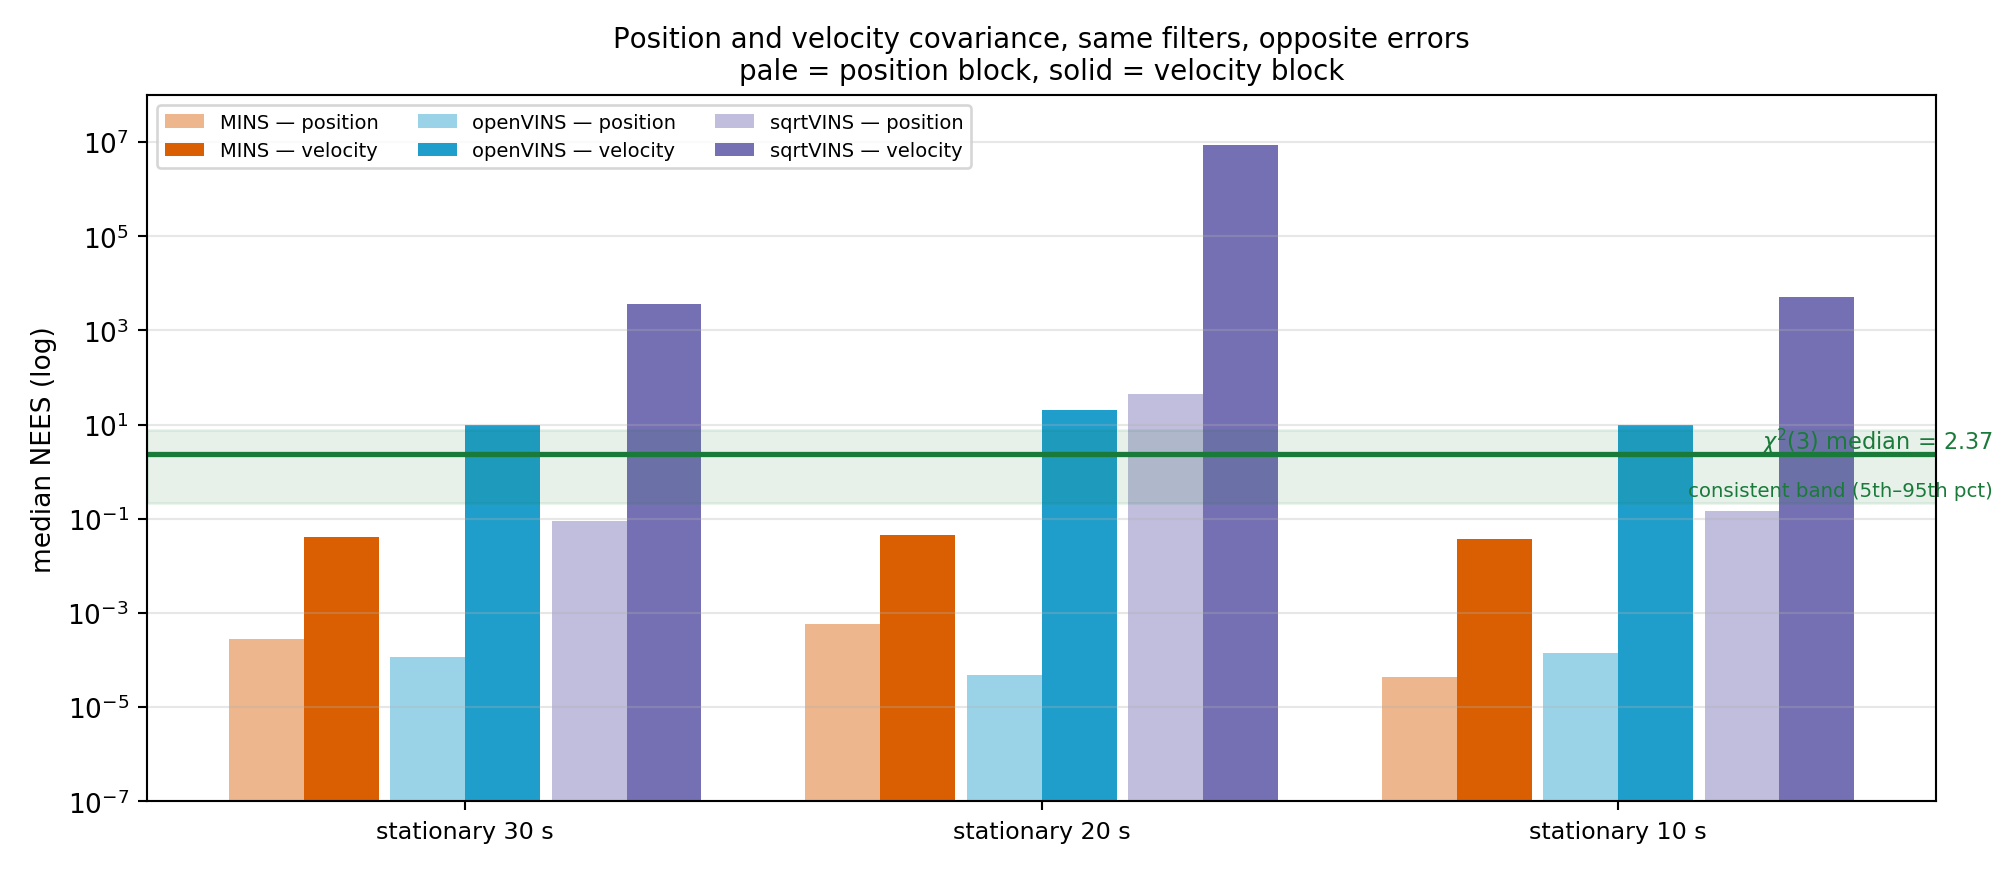
\includegraphics[width=\linewidth]{figures/nees_pos_vit.png}%
  }{%
    \fbox{\parbox{0.9\linewidth}{\centering\vspace{1em}
    \code{figures/nees\_pos\_vit.png} not generated\vspace{1em}}}%
  }
  \caption[Position and velocity covariance compared]{The two covariance
  blocks of each filter, on the same recordings. Pale bars are the position
  block, solid bars the velocity block; the green band spans the $5$th to
  $95$th percentiles of $\chi^2(3)$, within which a consistent filter should
  fall. MINS sits below it on both blocks, closer on velocity. openVINS
  falls far below on position and \emph{above} on velocity --- the same
  matrix wrong in opposite directions. sqrtVINS leaves the plot.}
  \label{fig:neesposvel}
\end{figure}

\subsection{The same matrix, wrong in opposite directions}
\label{sec:blocsopposes}

Placing the two blocks side by side is the result of this chapter:

\begin{center}
\begin{tabular}{@{}lrrl@{}}
\toprule
Estimator & $k$ (position) & $k$ (velocity) & \\
\midrule
MINS     & $0.004$--$0.016$ & $0.13$--$0.14$ & both conservative, velocity far less so \\
openVINS & $0.005$--$0.008$ & $\mathbf{2.03}$--$\mathbf{2.97}$ & \textbf{opposite signs} \\
sqrtVINS & $0.20$--$4.39$   & $38.8$--$1899$ & overconfident throughout \\
\bottomrule
\end{tabular}
\end{center}

\noindent openVINS is the striking case. Its position covariance is inflated
by a factor of roughly $150$ in $\sigma$, and its velocity covariance is
deflated by a factor of $2$ to $3$ --- two blocks of the same matrix,
published in the same message, erring in opposite directions. Nothing in the
pose alone reveals this; both blocks pass every check made earlier in this
report, because those checks never looked at $\mathbf{P}$.

The practical consequence follows from which block does what. A downstream
gate reading the position block will be far too permissive. Propagation
reading the velocity block will under-grow position uncertainty between
measurements, which partly explains why the position block can stay wide
while the filter's own predicted growth is too slow: the two errors are not
independent, they are the same miscalibration seen at two points of the same
loop.

\begin{trapbox}{Why this is worth more than a better tuned number}
The instinct on seeing $k=150$ is to divide the noise density by $150$ and
move on. That would be tuning to a single stationary recording and is
exactly the practice this report warns against elsewhere --- the same
mistake as inheriting a datasheet figure, with a different provenance.

What the measurement supports is narrower and more useful: a statement that
these covariances are \emph{not} calibrated, a number for how far, and a
procedure costing one stationary recording that can be repeated after any
change. A filter whose covariance is wrong by two orders of magnitude is not
producing an uncertainty estimate at all --- it is producing a constant that
happens to have units of metres, and the honest move is to say so rather
than to rescale it once and call it characterised.
\end{trapbox}

\subsection{The angular block, and what the three blocks say together}
\label{sec:neesangulaire}

The twist message carries angular velocity as well, and the stationary case
makes its truth exact for the same reason: a platform that does not move
does not rotate. Evaluating Eq.~(\ref{eq:neesvel}) on the
$\boldsymbol{\omega}$ block:

\begin{center}
\begin{tabular}{@{}llrrrr@{}}
\toprule
Recording & estimator & median $|\hat{\boldsymbol{\omega}}|$ & $\sigma_\omega$ & $\varepsilon_\omega$ & $k$ \\
\midrule
stationary 30\,s & MINS     & $0.137$ & $0.00126$ & $3.59$ & $\mathbf{1.23}$ \\
                 & openVINS & $0.137$ & $0.00323$ & $0.55$ & $0.48$ \\
                 & sqrtVINS & $0.094$ & $0.00323$ & $0.27$ & $0.34$ \\
\midrule
stationary 20\,s & MINS     & $0.140$ & $0.00126$ & $3.75$ & $\mathbf{1.26}$ \\
                 & openVINS & $0.139$ & $0.00324$ & $0.56$ & $0.49$ \\
                 & sqrtVINS & $0.095$ & $0.00324$ & $0.26$ & $0.33$ \\
\midrule
stationary 10\,s & MINS     & $0.144$ & $0.00126$ & $3.94$ & $\mathbf{1.29}$ \\
                 & openVINS & $0.145$ & $0.00324$ & $0.61$ & $0.51$ \\
                 & sqrtVINS & $0.095$ & $0.00325$ & $0.26$ & $0.33$ \\
\bottomrule
\end{tabular}
\end{center}

\noindent Angular rates in deg/s, $\sigma_\omega$ in rad/s.

\textbf{MINS's angular block is calibrated.} $k$ between $1.23$ and $1.29$
places its reported $\sigma$ within thirty per cent of what the error
warrants, and $\varepsilon_\omega$ between $3.59$ and $3.94$ sits close to
the $\chi^2(3)$ mean of $3$. After a position block wrong by two orders of
magnitude, this is the one covariance in the entire report that a consumer
could use as published.

Note also that all three estimators report ${\approx}0.14$\,deg/s of
residual angular rate on a platform that is not turning --- a direct
reading of the gyroscope bias surviving the sanitiser, and one the two
filters sharing \code{/imu/data\_clean} agree on to three digits.

\begin{figure}[htbp]
  \centering
  \IfFileExists{figures/gradient_covariance.png}{%
    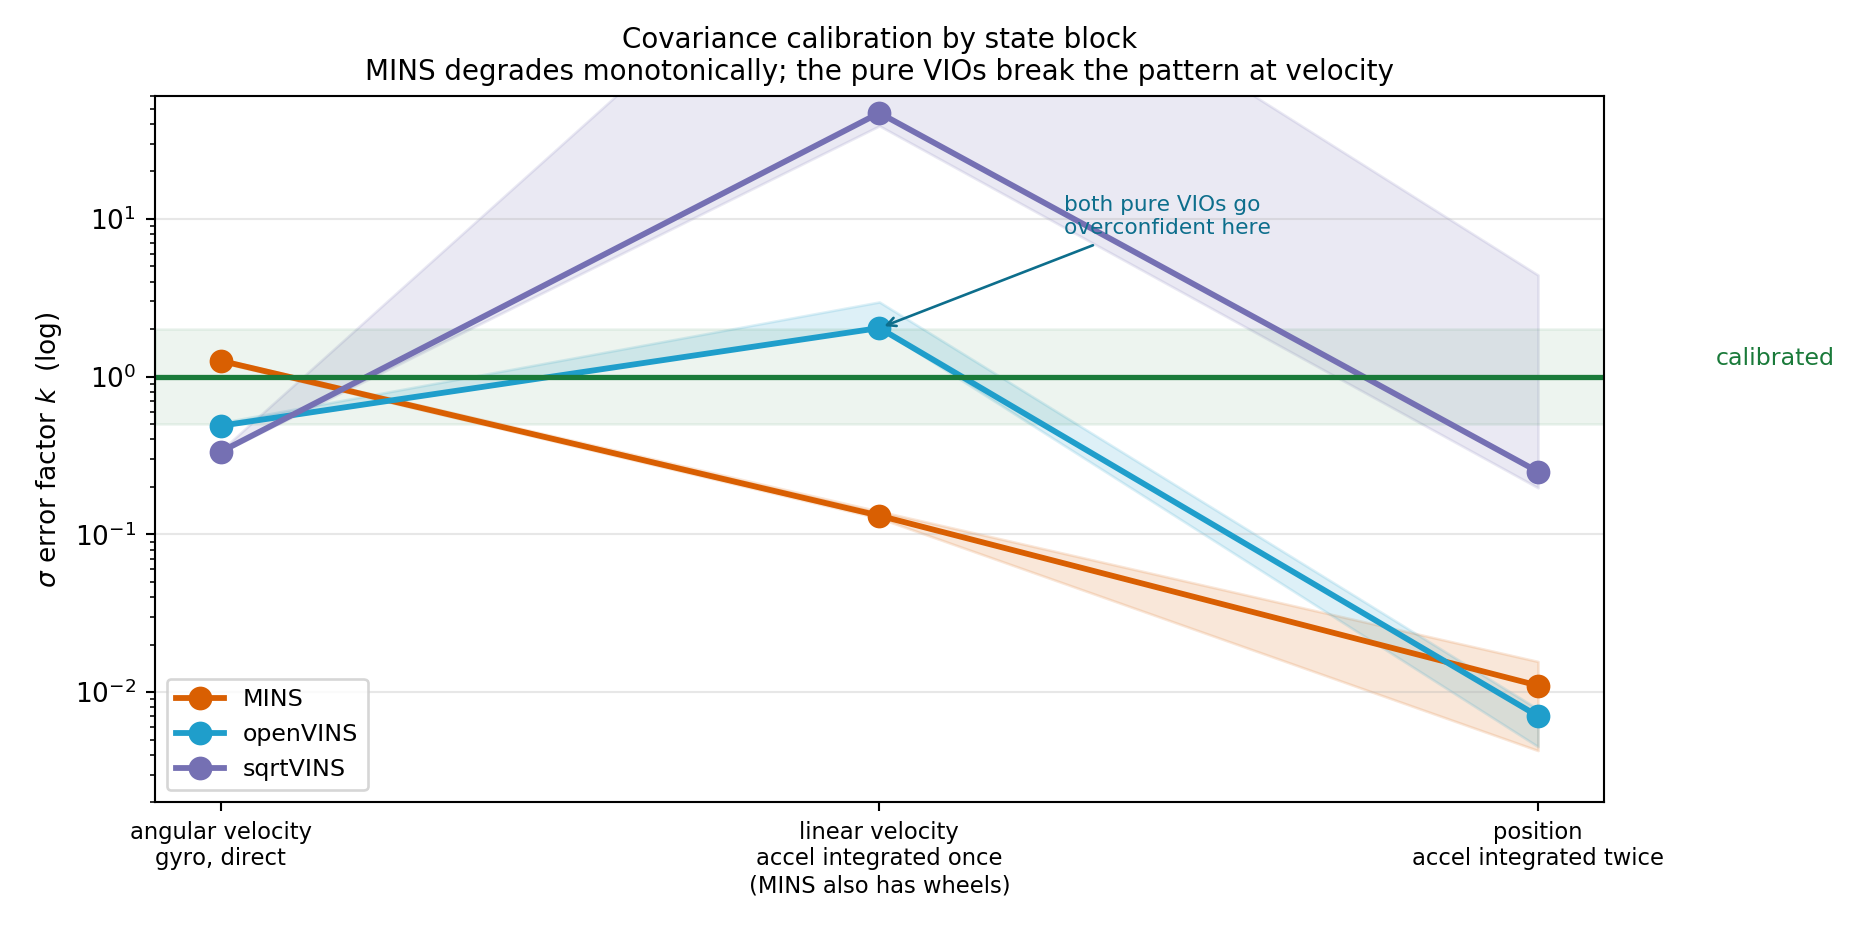
\includegraphics[width=\linewidth]{figures/gradient_covariance.png}%
  }{%
    \fbox{\parbox{0.9\linewidth}{\centering\vspace{1em}
    \code{figures/gradient\_covariance.png} not generated\vspace{1em}}}%
  }
  \caption[Covariance calibration across the three state blocks]{The
  $\sigma$ error factor $k$ of Eq.~(\ref{eq:sigmafactor}) for each state
  block, medians across the three stationary recordings with the shaded band
  giving their spread. Unity is calibrated. MINS declines monotonically from
  the directly measured angular rate to the twice-integrated position.
  The two pure VIO filters do not: both are overconfident precisely at
  linear velocity, the one channel for which MINS carries an independent
  measurement.}
  \label{fig:gradientcov}
\end{figure}

\paragraph{MINS degrades with integration depth; the others do not.}
Figure~\ref{fig:gradientcov} places the three blocks in order of how far
each sits from a direct measurement. MINS falls monotonically ---
$k = 1.26$ on the gyro-derived rate, $0.131$ after one integration,
$0.011$ after two --- losing about an order of magnitude per integration.
That is the behaviour one would predict: uncertainty about an integrated
quantity is dominated by the process-noise model, and modelling error
compounds with each integration.

The two pure VIO filters break that pattern, and both break it at the same
place. openVINS goes from $k=0.49$ on angular rate to $k=2.03$ on linear
velocity --- from conservative to overconfident in one step --- before
collapsing to $0.007$ on position. sqrtVINS does the same more violently,
$0.33 \rightarrow 46.9 \rightarrow 0.249$.

\begin{trapbox}{A plausible reading, offered as a hypothesis}
Linear velocity is the one block where MINS has something the other two do
not: a direct measurement from the wheels. A pure VIO must infer linear
velocity from integrated acceleration and visual parallax, with no sensor
observing it; MINS reads it from the encoders through the
\code{Wheel2DAng} model.

That the two filters lacking a velocity measurement are the two that go
overconfident on the velocity block is consistent, and it would explain why
the anomaly sits exactly there rather than anywhere else in the chain. It is
not established. Testing it would mean disabling MINS's wheel updater and
re-running the same measurement, which is a twenty-minute experiment and is
recorded here as the next thing to do rather than as a conclusion already
drawn.
\end{trapbox}

\subsection{A covariance that has stopped being a variable}
\label{sec:covsaturee}

The stationary recordings showed \emph{what} the covariances are worth. The
seven-minute drive shows \emph{how they behave}, and for MINS the answer is
that its position covariance stops behaving at all.

A filter propagating between corrections should see $\mathbf{P}$ grow, since
integrating IMU noise adds uncertainty; each accepted measurement should
pull it back. The published series should therefore saw-tooth. Sampling
MINS over the window $150 \le t \le 420$\,s --- $23{,}137$ samples, during
which the estimator itself reports $6.09$\,m of travel:

\begin{center}
\begin{tabular}{@{}lrr@{}}
\toprule
Window $150$--$420$\,s & MINS & openVINS \\
\midrule
$3\sigma$ minimum & $12.8908$\,m & $0.2600$\,m \\
$3\sigma$ maximum & $12.9255$\,m & $4.0005$\,m \\
range over $270$\,s & $\mathbf{0.0347}$\,\textbf{m} & $3.7405$\,m \\
coefficient of variation & $\mathbf{2.8\times10^{-4}}$ & $5.8\times10^{-1}$ \\
path reported over window & $6.09$\,m & $2307.61$\,m \\
\bottomrule
\end{tabular}
\end{center}

\noindent MINS's reported position uncertainty varies by three and a half
centimetres across four and a half minutes of driving --- three parts in ten
thousand. It is not a saw-tooth, not a growth curve, not a decay: it is a
constant that happens to be expressed in metres.

\begin{center}
\begin{tikzpicture}[font=\small, >={Latex[length=2mm]}, xscale=1.06]
  \draw[->, thick] (0,0) -- (9.2,0) node[right, font=\scriptsize] {$t$};
  \draw[->, thick] (0,0) -- (0,2.9) node[above, font=\scriptsize] {$3\sigma$};
  % attendu : dents de scie
  \draw[thick, green!45!black]
    (0.3,0.35) -- (1.3,1.15) -- (1.3,0.45) -- (2.3,1.25) -- (2.3,0.5)
    -- (3.3,1.3) -- (3.3,0.55) -- (4.1,1.2);
  \node[font=\scriptsize, text=green!35!black, anchor=west] at (0.35,1.62)
    {expected: grow, then a correction pulls it back};
  % observe : plat
  \draw[very thick, alertred!75] (4.9,0.95) -- (8.9,0.96);
  \node[font=\scriptsize, text=alertred!85, anchor=west] at (4.95,1.45)
    {observed on MINS: flat to $3\times10^{-4}$};
  \draw[dotted, gray] (4.5,0) -- (4.5,2.6);
  \node[font=\scriptsize, anchor=north] at (2.2,-0.12) {a filter tracking its own uncertainty};
  \node[font=\scriptsize, anchor=north] at (6.9,-0.12) {a filter reporting a ceiling};
\end{tikzpicture}
\end{center}

\subsection{Reading the two behaviours together}

The contrast with openVINS on the same window is what makes the point,
because the two failures are opposite and neither is visible from the pose
alone.

openVINS's covariance \emph{does} move --- a coefficient of variation of
$0.58$, a step from $0.26$ to $3.67$\,m around $t=230$\,s, genuine
structure. But over that same window it reports $2307$\,m of travel on a
platform that covered a few metres. Its covariance is alive and its state is
nonsense.

MINS is the mirror image. Its pose over that window is the only one of the
three that stays physically possible (\S\ref{sec:plafondphysique}), and its
covariance is inert. A consumer reading only the pose would prefer MINS
without hesitation; a consumer reading only the covariance would see a
number that never changes and conclude, wrongly, that nothing was happening.

\begin{trapbox}{What a saturated covariance costs, concretely}
Three consequences follow, and none of them show up as an error message.

\textbf{A $\chi^2$ gate built on it cannot reject.} The gate compares a
residual against $\mathbf{P}$; a $\mathbf{P}$ two orders of magnitude too
large accepts essentially any measurement, which removes the very protection
the gate exists to provide.

\textbf{Fusion weighting is wrong by the same factor.} Any node combining
this pose with another source weights by $\mathbf{P}^{-1}$, so MINS is
weighted a hundred times less than its accuracy deserves.

\textbf{Divergence becomes undetectable from the covariance.} A filter
losing its fix normally announces it by a growing $\mathbf{P}$. If
$\mathbf{P}$ is pinned at a ceiling, the two spontaneous divergences of
\S\ref{sec:openitems} --- item 47, still open --- would look identical to
healthy operation in the one channel designed to warn about them. That is
consistent with what was observed on 2026-09-08, where the failure was
found by reading $z$ directly and not by any covariance signal.
\end{trapbox}
